% !TEX program = xelatex
% Self-contained single-file build for Overleaf. COMPILER: XeLaTeX.
% Upload 6 images (project root or a figures/ subfolder): khtn_logo.png,
%   bc_fig1_main.pdf bc_fig2_discovery.pdf bc_fig3_ctc.pdf bc_fig4_epistemic.pdf bc_fig5_boundary.pdf
\documentclass[12pt,a4paper]{report}
\usepackage{fontspec}   % XeLaTeX: native Unicode (Vietnamese) rendering
\usepackage{lmodern}
\usepackage{amsmath,amssymb}
\usepackage{graphicx}
\graphicspath{{figures/}{./}{../figures/}}
\usepackage{booktabs,longtable,array,calc}
\usepackage{caption}
\usepackage{float}
\usepackage{microtype}
\usepackage[a4paper,top=2cm,bottom=2cm,left=2.5cm,right=2.5cm]{geometry}
\usepackage{tikz}
\usetikzlibrary{arrows.meta}
\usepackage{xcolor}
\usepackage[hidelinks]{hyperref}
\usepackage{parskip}
\usepackage{textcomp}
\usepackage{newunicodechar}
\newunicodechar{§}{\S}
\newunicodechar{·}{\textperiodcentered}
\newunicodechar{…}{\ldots}
\newunicodechar{–}{--}
\newunicodechar{—}{---}
\newunicodechar{°}{\textdegree}
\newunicodechar{±}{\ensuremath{\pm}}
\newunicodechar{×}{\ensuremath{\times}}
\newunicodechar{≈}{\ensuremath{\approx}}
\newunicodechar{≠}{\ensuremath{\neq}}
\newunicodechar{≥}{\ensuremath{\geq}}
\newunicodechar{≤}{\ensuremath{\leq}}
\newunicodechar{→}{\ensuremath{\rightarrow}}
\newunicodechar{←}{\ensuremath{\leftarrow}}
\newunicodechar{−}{\ensuremath{-}}
\newunicodechar{∇}{\ensuremath{\nabla}}
\newunicodechar{∅}{\ensuremath{\emptyset}}
\newunicodechar{△}{\ensuremath{\triangle}}
\newunicodechar{θ}{\ensuremath{\theta}}
\newunicodechar{π}{\ensuremath{\pi}}
\newunicodechar{α}{\ensuremath{\alpha}}
\newunicodechar{†}{\textdagger}
\newunicodechar{⚠}{\textbf{!}}

\usepackage{listings}
\lstset{basicstyle=\ttfamily\footnotesize,breaklines=true,breakatwhitespace=false,
  columns=fullflexible,keepspaces=true,showstringspaces=false,frame=none,
  breakindent=0pt,postbreak=\mbox{\textcolor{gray}{$\hookrightarrow$}\space}}
\usepackage{etoolbox}
\AtBeginEnvironment{longtable}{\small}
\AtBeginEnvironment{verbatim}{\footnotesize}

\providecommand{\tightlist}{\setlength{\itemsep}{0pt}\setlength{\parskip}{0pt}}
\providecommand{\passthrough}[1]{#1}
\providecommand{\pandocbounded}[1]{#1}
\providecommand{\real}[1]{#1}

\setcounter{secnumdepth}{3}
\setcounter{tocdepth}{2}

% compact chapter headings (less blank space at the top of chapter/appendix pages)
\usepackage{titlesec}
\titleformat{\chapter}[display]{\normalfont\bfseries\Huge}{\chaptertitlename\ \thechapter}{6pt}{\Huge}
\titlespacing*{\chapter}{0pt}{4pt}{16pt}

\begin{document}

% ============================ TITLE PAGE ============================
\begin{titlepage}
\centering
{\large\bfseries UNIVERSITY OF SCIENCE - VNUHCM\par}
{\bfseries Faculty of Mathematics and Computer Science\par}
{\bfseries Major of Data Science\par}
\vspace{1.0cm}

\includegraphics[width=3.3cm]{khtn_logo.png}\par
\vspace{1.4cm}
{\large\bfseries Graduation Thesis\par}
\vspace{1.1cm}
{\Large\bfseries Accelerating Test-Time Discovery in Complex Code Generation via Execution-Guided Self-Distillation\par}
\vspace{2.4cm}
\begin{flushleft}\large
\begin{tabular}{l|l}
Student & Student ID\\ \hline
Mai Phong Đăng & 22280008\\
\end{tabular}\\[0.6em]
Course 2022
\end{flushleft}
\vspace{0.5cm}
\begin{flushright}\large
Supervisor: Dr.\ Ngô Minh Mẫn
\end{flushright}
\vfill
{\large Ho Chi Minh City, 2026\par}
\end{titlepage}

\chapter*{Abstract}
\addcontentsline{toc}{chapter}{Abstract}
Test-time training lets a language model improve on a single hard
problem at inference time, but on-policy self-distillation stalls when
the model rarely produces a correct attempt to learn from. This thesis
studies how to accelerate test-time discovery in complex code generation
via \emph{execution-guided self-distillation}, where execution feedback
(failing tests, runtime errors) is the privileged context that drives
the update. We propose a \emph{teacher-first} organization: rather than
distilling the student's own failed rollout, the self-teacher generates
trajectories under feedback, a verifier and a judge filter them for
correctness and independence, and the student is distilled toward those
filtered trajectories, placing the method between on-policy SDPO and
off-policy SFT. Across a medium-sized matched evaluation on hard
LiveCodeBench problems with a 4B model, teacher-first significantly
outperforms the student-first baseline (Wilcoxon signed-rank), and on
the hardest problems it escapes the flat-reward trap that keeps
student-first stuck at zero. A compute-matched comparison shows the
advantage is not a sampling-volume artifact: at equal generation budget
teacher-first still wins, and reaches a given discovery probability with
fewer total generations. With thinking enabled, we measure epistemic
verbalization at test time and find that distillation from a
feedback-conditioned context suppresses uncertainty markers, connecting
the method to the degradation Kim et al.~describe. Finally, evaluating the
pipeline on mathematical reasoning (AIME 2026) exposes a rigid domain
boundary: when feedback is limited strictly to a static numeric value
rather than an algorithmic procedure, the teacher policy degrades into
shallow answer-copying without capability lift, establishing a strict
procedural-versus-value constraint on test-time self-distillation.

\vspace{0.5cm}
\textbf{Keywords:} test-time training, self-distillation, code
generation, execution feedback, discovery@k, epistemic suppression,
domain boundary.

\tableofcontents

\clearpage
\addcontentsline{toc}{chapter}{List of Figures}
\listoffigures

\clearpage
\addcontentsline{toc}{chapter}{List of Tables}
\listoftables

\chapter{Introduction}\label{chapter-1-introduction}

This thesis studies how to accelerate test-time discovery in complex code generation via execution-guided self-distillation. The core question is practical: when a language model is given a single hard programming problem and a budget to improve itself at inference time, what is the most effective way to turn execution feedback into a better solution, and when does that strategy work?

\section{Background}\label{background}

Reinforcement learning with verifiable rewards (RLVR), with GRPO {[}8{]} as a common instantiation, suffers from sparse credit assignment: a scalar outcome reward says only whether an attempt passed, and when every rollout fails the advantage collapses and learning stalls --- exactly on the hard problems that matter. Self-Distillation Policy Optimization (SDPO) {[}1{]} extracts a denser signal from the rich feedback verifiable environments already produce, using the feedback-conditioned model as a self-teacher distilled back into the student. At test time it can iterate on one hard problem and improve before the first success {[}1, §5{]}. Two issues motivate this work: the parent paper distills the student's own failed rollout (little that is correct to learn from on hard problems), and Kim et al.~{[}2{]} show that distilling from rich context can degrade a model by suppressing its epistemic verbalization.

\section{Problem}\label{problem}

The setting is test-time training: one hard problem, a verifiable reward, a short budget of self-improvement steps, then reset. Two design choices govern discovery: how the execution feedback is organized into a learning signal (learn from the student's failed attempt, or from a correct attempt produced under feedback and filtered for independence), and how the execution feedback is formulated into the reprompt the self-teacher sees {[}1, §7{]}. We take execution feedback as the privileged context, hence \emph{execution-guided}, and study both choices with the goal of accelerating discovery.

\section{Research questions}\label{research-questions}

\begin{itemize}
\tightlist
\item
  \textbf{RQ-method.} Does a teacher-first organization beat the student-first baseline at discovering solutions to hard code problems, and does the advantage survive at matched compute?
\item
  \textbf{RQ1.} Does the reprompt-template formulation of the execution feedback affect discovery, and in which regime?
\item
  \textbf{RQ2.} Does self-distillation from rich context suppress epistemic verbalization at test time on code?
\item
  \textbf{RQ3.} What are the structural and domain limitations of execution-guided self-distillation when transitioning from procedural code to value-only mathematical contexts?
\end{itemize}

All four research questions are systematically evaluated and addressed throughout the empirical framework of this thesis.

\section{Contributions}\label{contributions}

\begin{enumerate}
\def\labelenumi{\arabic{enumi}.}
\tightlist
\item
  \textbf{A teacher-first variant of execution-guided self-distillation} that distills the student toward verifier- and judge-filtered teacher generations, between on-policy SDPO and off-policy SFT, with a clean filter that never distils a copy (Chapter 3).
\item
  \textbf{Teacher-first significantly accelerates discovery in code, and the advantage is compute-fair.} Across a matched evaluation ($8\text{ problems} \times 6\text{ seeds}$), teacher-first beats student-first (Wilcoxon signed-rank) and escapes the flat-reward trap on the hardest problems; a compute-matched comparison and a compute-to-correct frontier show the gain is not a sampling-volume artifact (Chapter 4).
\item
  \textbf{A reprompt-template effect}, strongest on hard problems, where a reasoning-inducing template orders above the anchor, which orders above a minimal one (§4.5).
\item
  \textbf{A measured epistemic-suppression result on code} (thinking enabled): distillation from a feedback-conditioned context suppresses uncertainty markers, accumulating across steps (§4.7).
\item
  \textbf{A characterized value-versus-procedure domain boundary.} By demonstrating that the pipeline falls into an inescapable zero-reward trap on AIME 2026, we empirically isolate a fundamental limit of the approach: self-distillation requires a procedure-bearing learning signal (like dense code test cases) to internalize methods, and stalls when restricted to static, value-only references (§4.8, Chapter 5).
\end{enumerate}

\section{Scope}\label{scope}

Test-time training with LoRA adapters; complex code generation on LiveCodeBench v6 {[}6{]} serves as the core empirical domain, with AIME 2026 deployed as the contrasting mathematical baseline environment. Results are centered on a 4B-scale reasoning model family. The study remains an empirical characterization within a personal compute scale, establishing clear domain boundaries and foundational insights rather than claiming universal scaling laws.

\section{Thesis structure}\label{thesis-structure}

Chapter 2 reviews background and related work; Chapter 3 specifies the method (including the thinking-on extensions); Chapter 4 reports the multi-seed code experiments, the compute-matched comparison, the epistemic-suppression result, and the mathematical domain boundary; Chapter 5 discusses the underlying mechanisms; Chapter 6 states the remaining structural limitations and the publication roadmap; Chapter 7 concludes.
\chapter{Background and Related Work}\label{chapter-2-background-and-related-work}

This chapter sets out the background the thesis builds on. It moves from the reinforcement-learning setting that motivates self-distillation (§2.1), through the SDPO method and its loss (§2.2), to the test-time regime and its metric (§2.3), the reprompt-template design space (§2.4), the epistemic-suppression critique (§2.5), and a sister self-distillation method (§2.6), closing with the gap this thesis addresses (§2.7).

\section{RLVR and GRPO}\label{rlvr-and-grpo}

Reinforcement learning with verifiable rewards (RLVR) is the dominant post-training recipe for code and math, where an automatic checker supplies the reward. Group Relative Policy Optimization (GRPO) {[}8{]} is a common instantiation: it samples a group of rollouts per problem and assigns each an advantage relative to the group mean, \(A_{i,t} = r_i - \text{mean}_j\{r_j\}\), which is constant across the tokens of a sequence.

GRPO is attractive because it removes the separate value network of PPO-style methods: the group mean serves as the baseline, and the advantage is estimated from the spread of rewards within the sampled group {[}8{]}. This keeps the method simple and is part of why it became the default for verifiable domains.

The same simplicity is its structural weakness in credit assignment. A scalar outcome reward records only whether a rollout passed, not which tokens were responsible, so the learning signal is sparse {[}1{]}. The weakness becomes a failure when every rollout in a group fails: the group-relative advantage collapses to zero and no gradient flows, so the method cannot learn on a problem until it has already solved it at least once. Hard problems, where successes are rare, are precisely where this stalls.

A natural fix is to distill from a stronger teacher, but that requires a teacher more capable than the student, which is unavailable when the goal is to raise the capability ceiling rather than to compress a known one {[}1{]}. This tension motivates a teacher that is not external but derived from the student itself.

\section{SDPO}\label{sdpo}

\subsection{The self-teacher and rich feedback}\label{the-self-teacher-and-rich-feedback}

Hübotter et al.~{[}1{]} observe that many verifiable environments already expose tokenized feedback, such as runtime errors, failing-test diffs, or judge comments, which is discarded when the signal is collapsed to a scalar reward. They propose reinforcement learning with rich feedback (RLRF) as a framework that keeps this signal, and SDPO as its instantiation. The mechanism that makes it possible is in-context learning: the same model, conditioned on the feedback \(f\) in addition to the question \(x\), can often locate its own mistake. This conditioned model, \(\pi_\theta(\cdot \mid x, f)\), serves as a \emph{self-teacher}, while the unconditioned \(\pi_\theta(\cdot \mid x)\) is the student. Both share the weights \(\theta\), so this is self-distillation in the lineage of knowledge distillation {[}13{]}, but with feedback rather than a larger network as the source of the teacher's advantage.

\subsection{The loss and dense credit assignment}\label{the-loss-and-dense-credit-assignment}

SDPO distills the self-teacher's retrospective next-token distribution into the student by a per-token KL:

\[
\mathcal{L}_{\text{SDPO}}(\theta) = \sum_{t=1}^{|y|} \mathrm{KL}\,\Big(\pi_\theta(\cdot \mid x, y_{<t}) \,\big\|\, \mathrm{stopgrad}\,\pi_\theta(\cdot \mid x, f, y_{<t})\Big),
\]

where \passthrough{\lstinline!stopgrad!} prevents the teacher from collapsing onto the student to ignore \(f\) {[}1{]}. With the teacher detached, the gradient at a student logit is \(\partial\mathcal{L}/\partial z_v = \pi_S(v) - \pi_T(v)\), so the optimizer raises every logit the teacher trusts more than the student does. The contrast with GRPO is the density of the target:

\begin{longtable}[]{@{}
  >{\raggedright\arraybackslash}p{(\columnwidth - 4\tabcolsep) * \real{0.3333}}
  >{\raggedright\arraybackslash}p{(\columnwidth - 4\tabcolsep) * \real{0.3333}}
  >{\raggedright\arraybackslash}p{(\columnwidth - 4\tabcolsep) * \real{0.3333}}@{}}
\caption{Credit-assignment density: per-token target for GRPO versus SDPO.}\\
\toprule\noalign{}
\begin{minipage}[b]{\linewidth}\raggedright
Method
\end{minipage} & \begin{minipage}[b]{\linewidth}\raggedright
Target per token
\end{minipage} & \begin{minipage}[b]{\linewidth}\raggedright
Signal per sequence
\end{minipage} \\
\midrule\noalign{}
\endfirsthead
\toprule\noalign{}
\begin{minipage}[b]{\linewidth}\raggedright
Method
\end{minipage} & \begin{minipage}[b]{\linewidth}\raggedright
Target per token
\end{minipage} & \begin{minipage}[b]{\linewidth}\raggedright
Signal per sequence
\end{minipage} \\
\midrule\noalign{}
\endhead
\bottomrule\noalign{}
\endlastfoot
GRPO & scalar advantage × one-hot & \(O(1)\) \\
SDPO (sequence-level) & scalar × soft distribution & \(O(1)\) \\
SDPO (token-level) & soft distribution, top token & \(O(T)\) \\
SDPO (logit-level) & soft distribution over top-\(K\) vocab & \(O(T \cdot K)\) \\
\end{longtable}

\begin{figure}[H]
\centering
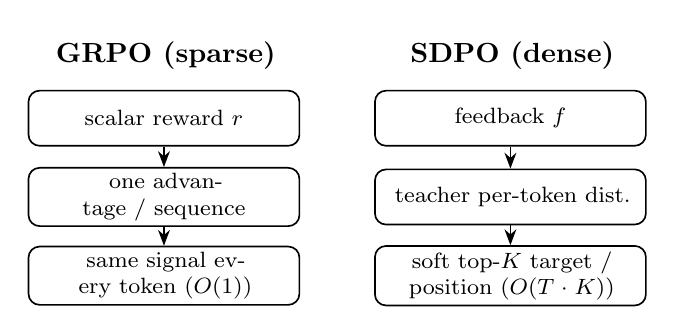
\begin{tikzpicture}[font=\footnotesize,>=Stealth,semithick,every node/.style={draw,rounded corners,align=center,minimum height=0.7cm,text width=3.3cm,inner sep=2pt}]
\node(gr) at (0,3){scalar reward $r$};
\node(ga) at (0,2){one advantage / sequence};
\node(gt) at (0,1){same signal every token ($O(1)$)};
\node(sf) at (4.4,3){feedback $f$};
\node(st) at (4.4,2){teacher per-token dist.};
\node(stk) at (4.4,1){soft top-$K$ target / position ($O(T\cdot K)$)};
\draw[->](gr)--(ga);\draw[->](ga)--(gt);\draw[->](sf)--(st);\draw[->](st)--(stk);
\node[draw=none,font=\bfseries] at (0,3.8){GRPO (sparse)};
\node[draw=none,font=\bfseries] at (4.4,3.8){SDPO (dense)};
\end{tikzpicture}
\caption{Credit-assignment density, GRPO versus SDPO. GRPO attaches one scalar advantage to a whole sequence, so every token receives the same signal (\(O(1)\)); SDPO conditions the teacher on feedback and supplies a soft, \(K\)-dimensional target per position (\(O(T\cdot K)\)).}
\label{fig:credit-density}
\end{figure}

The full method is logit-level: the target is a \(K\)-dimensional distribution at every position rather than a single scalar per sequence, which is the source of its sample efficiency {[}1{]}. To keep this affordable at a vocabulary of roughly 150k, only the teacher's top-\(K\) logits (with \(K{=}100\), or 20 for the code configuration {[}4{]}) plus a tail bucket are kept. The KL direction is parameterized by \(\alpha\): forward KL (\(\alpha{=}0\)) is mode-covering, reverse KL (\(\alpha{=}1\)) is mode-seeking, and JSD (\(\alpha{=}0.5\)) interpolates, the last following Agarwal et al.~{[}11{]} for stability. The self-teacher is regularized, typically by an EMA of the student weights or a trust-region interpolation, since an unregularized teacher diverges {[}1{]}. The implementation used in this thesis is specified in §3.3.5; the derivation is consolidated in the project notes.

\subsection{Three regimes}\label{three-regimes}

The parent paper validates SDPO across three settings. In a plain RLVR setting without native rich feedback, it manufactures feedback by using a successful in-batch rollout as the reference for a failed one, and still beats GRPO substantially, reaching a GRPO five-hour accuracy in fifty minutes on one chemistry task {[}1{]}. In the RLRF setting with genuine code-execution feedback on LiveCodeBench v6 {[}6{]}, it reports 48.8\% versus GRPO's 41.2\% and matches GRPO's final accuracy with roughly 4× fewer generations. The third setting, test-time discovery on hard problems, is the regime this thesis works in and is treated next.

\subsection{What drives SDPO: ablations and scaling}\label{what-drives-sdpo-ablations-and-scaling}

Three findings from the parent paper's analysis bear directly on the choices made in this thesis.

First, both ingredients of SDPO matter. Decomposing the method into logit-level, token-level, and sequence-level variants gives an ordering logit \textgreater{} token \textgreater{} sequence \textgreater{} GRPO {[}1, §4.2{]}, which shows that rich feedback and dense credit assignment each contribute rather than one carrying the result. A feedback-type ablation (its Table 6) is equally pointed: the environment output alone reaches 39.9\% training accuracy and the model's own prior solution alone 42.6\%, while combining them reaches 48.3\%, so the two are complementary. Adding the student's own failed attempt to the teacher context, by contrast, drops accuracy to 44.5\% and lowers entropy by 0.23, because the teacher is biased toward the student and loses diversity. This last result is part of the motivation for the teacher-first organization of §3.3, which distills filtered teacher generations rather than the student's failed attempt.

Second, self-teaching is emergent with scale {[}1, §4.1{]}. On Qwen3-8B, SDPO far exceeds GRPO; on Qwen3-0.6B the two are comparable; and on Qwen2.5-1.5B, SDPO underperforms GRPO. The method needs in-context learning strong enough for the conditioned model to act as a useful teacher. This places the 4B model used here in a band where SDPO is expected to work, and it also predicts that on a stronger model the student-first baseline should improve on its own, narrowing the teacher-first margin, a prediction revisited in Chapter 6.

Third, the self-teacher is bootstrapped, not fixed. It updates alongside the student and its accuracy rises during training, and the final student exceeds the initial teacher, so the method is not capped by the teacher it starts with {[}1, §4.3{]}. Regularization is what keeps this stable: a trust-region teacher (50.6\%) edges out an EMA teacher (49.3\%) and a frozen one (48.8\%), while an unregularized teacher diverges. SDPO also forgets less than supervised fine-tuning on the self-teacher's outputs across held-out benchmarks, though slightly more than GRPO, indicating that the on-policy character of the update helps preserve prior capability {[}1, §4.4{]}. A hybrid that blends GRPO and SDPO advantages helps weak models but not strong ones {[}1, §4.5{]}.

\section{Test-time training and discovery@k}\label{test-time-training-and-discoveryk}

In the test-time setting {[}1, §5{]}, a single hard problem is fixed, the reward is binary, and the model must discover a solution as quickly as possible. Rather than concatenating a growing history into the context, as multi-turn reprompting does, SDPO compresses the feedback into the weights by distilling \(\pi_\theta(\cdot \mid x, c)\) into \(\pi_\theta(\cdot \mid x)\), which sidesteps the context-window limit.

The metric is discovery@k {[}1, Def. 5.1{]}, the probability of solving within the first \(k\) attempts, \(P(T \le k)\) with discovery time \(T = \min\{k : r(y_k) = 1\}\). It generalizes pass@k {[}9{]} from i.i.d. sampling to sequential algorithms that share state or update weights between attempts, and it reduces to pass@k when the algorithm is plain best-of-k. The lineage is the time-to-termination performance profile of Dolan and Moré {[}12{]}. Empirically, SDPO discovers 53.2\% of very-hard problems against best-of-k's 41.5\%, and on some problems is the only method to solve at all, even though the initial self-teacher accuracy is below 1\% on almost every hard problem {[}1{]}. That last point matters most: dense credit assignment lets the model improve before it has produced a single success.

\section{The reprompt template and its design space}\label{the-reprompt-template-and-its-design-space}

The self-teacher's behavior is controlled by the template that formats \(x\) and \(f\) into its context. The parent paper uses a slot-based template (its Table 2) that inserts a successful previous rollout, the environment feedback, and a closing directive, and reports that performance is ``not sensitive to syntactic variations'' of this template, while the feedback type does matter: an ablation (its Table 6) finds the environment output and the model's own solution to be complementary, and including the student's own failed attempt in the teacher context reduces diversity {[}1{]}.

Two gaps follow. The paper tests syntactic variation but not semantic or instructional variation, and it explicitly names systematic study of how the reprompt template influences behavior as future work {[}1, §7{]}. This thesis organizes the template design space along three dimensions: information content, motivated by Kim et al.'s finding that context richness governs suppression {[}2{]}; instruction framing, addressing the open question above; and memory depth, motivated by the sequential accumulation of the test-time setting. The seven templates of §3.4 sample points across these dimensions, with the paper's default as the anchor.

\section{Epistemic verbalization and suppression}\label{epistemic-verbalization-and-suppression}

Kim et al.~{[}2{]} supply the cautionary counterpart to SDPO. They show that distilling from a rich context can degrade a model by suppressing its \emph{epistemic verbalization}, the uncertainty markers such as ``wait'' or ``maybe'' that accompany genuine reasoning. Their analysis ties the magnitude of suppression to the mutual information \(I(y; c \mid x)\) between the output and the context: the richer the context, the stronger the suppression. They probe the spectrum by varying what the teacher context contains, from nothing (\(c = \varnothing\)), through a solution stripped of its thinking and a regenerated answer, to a full solution, and find suppression growing with the information the context carries. The effect accumulates across successive distillation steps, and they recommend freezing the teacher (no EMA update) to break the feedback loop, in tension with the parent paper's preference for a moving, regularized teacher (§2.2.4).

For this thesis the relevance is twofold. The suppression risk is sharpest exactly when the context contains the answer, which is the math leak regime studied in the pilot (§4.9), where the teacher can copy the answer rather than derive it. And the accumulation across steps is precisely what the test-time setting applies repeatedly, since each TTT step distills again from the same answer-bearing context.

\section{SDFT and the leak concern}\label{sdft-and-the-leak-concern}

Shenfeld et al.~{[}3{]} propose self-distillation fine-tuning (SDFT) for continual learning, an on-policy, minimum-change distillation toward the model's own conditioned generation. It is a sister method: like SDPO it uses the model as its own teacher, but its aim is to preserve prior capability while adapting, which makes minimizing unintended change a design goal. The teacher-first organization of this thesis sits near SDFT in that it distills toward filtered model-generated trajectories, but it uses execution feedback as the conditioning context rather than a fixed demonstration (§3.3.1). SDFT's minimum-change framing also sharpens the leak question: if distillation transfers more than the intended content, what exactly is being copied, which is the question the math pilot answers concretely.

\section{The gap this thesis addresses}\label{the-gap-this-thesis-addresses}

The parent paper studies a student-first, on-policy SDPO, focuses its analysis on the train-time regimes, and reaches the test-time setting without studying the reprompt template there or measuring epistemic behavior. Kim et al.~characterize epistemic suppression but not in the test-time code-discovery setting. Shenfeld et al.~minimize change for continual learning rather than maximize discovery on a single hard problem. The gap, then, is threefold. First, a teacher-first organization of execution-guided self-distillation that distills filtered teacher generations, positioned between SDPO and SFT, and the question of whether it accelerates test-time discovery (RQ-method). Second, the effect of the reprompt-template formulation on that discovery, the open question the parent paper names (RQ1). Third, a characterization of when the approach helps, framed as the value-versus-procedure boundary that the code-versus-math contrast exposes. The remainder of the thesis addresses these in turn.

\chapter{Method}\label{chapter-3-method}

This chapter specifies the method in enough detail to reproduce it. The object of study is test-time SDPO {[}1, §5{]}: a single hard problem is fixed, the model improves itself over a small number of training steps at inference time (test-time training, TTT), and we measure how well it discovers a solution. Because the privileged context that drives the update is execution feedback (failing tests, runtime errors), we call this regime execution-guided self-distillation, and the goal is to accelerate that test-time discovery in complex code generation. Within the regime, the thesis contrasts two ways of organizing the update, student-first (the baseline of the originating paper {[}1{]}) and teacher-first (a variant proposed by the advisor), and then studies how the reprompt template formulates the execution feedback (RQ1).

Domain scope is asymmetric by design. Code generation is the core (LiveCodeBench v6 {[}6{]}); math is a pilot and a contrast (AIME 2026 {[}10{]}), used to characterize the boundary of the mechanism rather than to prove it works everywhere. That split is kept consistent throughout: every math setting carries the corresponding model and reference caveats (§3.5, Chapter 6).

Notation mirrors the parent paper, Hübotter et al.~{[}1{]}, so the two can be read side by side.

\begin{center}\rule{0.5\linewidth}{0.5pt}\end{center}

\section{Test-time SDPO pipeline}\label{test-time-sdpo-pipeline}

\subsection{Notation and setting}\label{notation-and-setting}

Fix a problem \(x\) (the problem statement). Two policies share the same weights \(\theta\):

\begin{itemize}
\tightlist
\item
  the student \(\pi_\theta(\cdot \mid x)\), which sees only the problem, and
\item
  the self-teacher \(\pi_\theta(\cdot \mid x, c)\), the same model conditioned on an additional privileged context \(c\).
\end{itemize}

In SDPO, \(c\) plays the role of the ``feedback'' \(f\) in the parent paper: retrospective information (a runtime error, a failing test, or a reference solution) that lets the model look back and locate its mistake {[}1, §2{]}. Because teacher and student differ only in their input context, this is genuine \emph{self}-distillation: the model learns by pulling its next-token distribution (without context) toward its own distribution conditioned on \(c\).

The test-time setting follows Hübotter et al.~{[}1, §5{]}. For each problem \(x\), the model is reset to a base checkpoint and then runs \(K\) TTT steps on that problem alone. The reward is verifiable, graded for code and binary for math. The goal is not to generalize to other problems but to discover a solution to \(x\) as early as possible; the metric is discovery@k {[}1, Def. 5.1{]} (§3.6).

\subsection{The shared loop}\label{the-shared-loop}

Both arms share one skeleton. The single thing that differs between them is \emph{which trajectories are distilled}:

\begin{lstlisting}
load base model + LoRA + optimizer (AdamW, lr = 1e-5)
PRE-eval (student pi_theta(*|x) only, N_eval samples)        # baseline
for step in 1..K:
    feedback        <- build_feedback(student attempt, verifier)   # rich feedback
    {trajectories}  <- generate(...)                               # arm-specific
    {distill_targets} <- select(...)                               # arm-specific (the core difference)
    if distill_targets != {}:
        theta <- theta - lr * grad_theta L_KL(distill_targets)                    # one optimizer step
    log step stats -> W&B
POST-eval (student pi_theta(*|x) only, N_eval samples)       # after TTT
report PRE->POST and the discovery curve
\end{lstlisting}

Figure~\ref{fig:two-arms} sketches the two arms; they diverge only at the shaded block.

\begin{figure}[H]
\centering
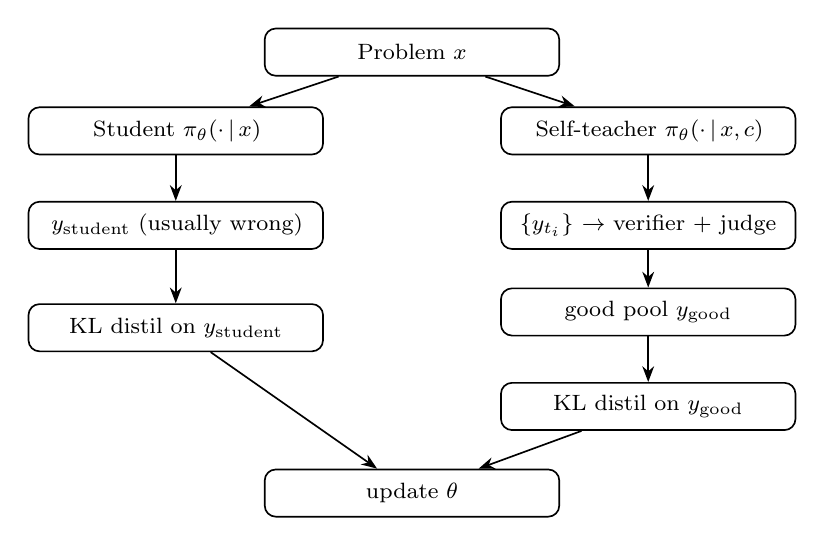
\begin{tikzpicture}[font=\footnotesize,>=Stealth,semithick,every node/.style={draw,rounded corners,align=center,minimum height=0.6cm,text width=3.6cm,inner sep=2pt}]
\node(x) at (3,5){Problem $x$};
\node(s) at (0,4){Student $\pi_\theta(\cdot\,|\,x)$};
\node(t) at (6,4){Self-teacher $\pi_\theta(\cdot\,|\,x,c)$};
\node(ys) at (0,2.8){$y_{\text{student}}$ (usually wrong)};
\node(yt) at (6,2.8){$\{y_{t_i}\}\to$ verifier + judge};
\node(g) at (6,1.7){good pool $y_{\text{good}}$};
\node(kls) at (0,1.5){KL distil on $y_{\text{student}}$};
\node(klt) at (6,0.5){KL distil on $y_{\text{good}}$};
\node(u) at (3,-0.6){update $\theta$};
\draw[->](x)--(s);\draw[->](x)--(t);\draw[->](s)--(ys);\draw[->](t)--(yt);\draw[->](yt)--(g);\draw[->](ys)--(kls);\draw[->](g)--(klt);\draw[->](kls)--(u);\draw[->](klt)--(u);
\end{tikzpicture}
\caption{The two arms of test-time SDPO. Student-first and teacher-first share the whole loop and diverge only at which trajectory is distilled (the shaded block).}
\label{fig:two-arms}
\end{figure}

The whole contrast reduces to one sentence: student-first distills the student's own failed attempt; teacher-first distills a correct, filtered trajectory generated by the teacher. Everything else (loss, model, hyperparameters) is held fixed to isolate that one variable.

\begin{center}\rule{0.5\linewidth}{0.5pt}\end{center}

\section{Student-first SDPO (baseline, on-policy)}\label{student-first-sdpo-baseline-on-policy}

This is the original algorithm of Hübotter et al.~{[}1{]}, realized through the \passthrough{\lstinline!SDPOTrainer!} of TRL {[}5{]} (script \passthrough{\lstinline!07\_discovery\_curve.py!}).

At each step the student samples a rollout \(y \sim \pi_\theta(\cdot \mid x)\) on-policy. The verifier grades \(y\) and produces feedback \(f\). The self-teacher \(\pi_\theta(\cdot \mid x, f)\) then rescores \emph{every token} of that same \(y\): given \(f\), what should the correct next-token distribution have been at each position? The student is pulled toward this retrospective distribution by a per-token KL:

\[
\mathcal{L}_{\text{SDPO}}(\theta) \;=\; \sum_{t=1}^{|y|} \mathrm{KL}\,\Big(\pi_\theta(\cdot \mid x, y_{<t}) \;\big\|\; \mathrm{stopgrad}\,\pi_\theta(\cdot \mid x, f, y_{<t})\Big).
\]

The \passthrough{\lstinline!stopgrad!} blocks gradient flow through the teacher, which prevents the teacher from collapsing onto the student and ignoring \(f\) {[}1, §2{]}. The gradient and the top-K approximation are shared with teacher-first and are deferred to §3.3.5.

There is a failure mode on hard problems that motivates the whole next section. Because rollouts are on-policy, on a problem the bare student rarely solves, almost every rollout is wrong, so the feedback is poor and the distillation signal is weak and unstable. This is the flat-reward trap: there is no correct rollout to learn from. Hübotter et al.~{[}1, §5{]} show SDPO can still iterate from rich feedback even when initial teacher accuracy is below 1\%, but they use Qwen3-8B; on the weaker 4B model used here (§3.5), the stuck-at-zero behavior does appear, and it is exactly what teacher-first targets.

\begin{center}\rule{0.5\linewidth}{0.5pt}\end{center}

\section{Teacher-first SDPO (proposed)}\label{teacher-first-sdpo-proposed}

\subsection{Motivation}\label{motivation}

Two problems with student-first motivate the variant.

First is the flat-reward trap of §3.2: when the student never rolls a correct attempt, there is nothing correct to distill.

Second is information leak {[}2{]}. If \(c\) contains a reference solution, the teacher rescores toward ``close to the reference,'' so across many test-time steps the student converges onto \emph{copying} the reference rather than learning to reason. Kim et al.~{[}2{]} formalize this: when \(I(y; c \mid x)\), the information richness of the context, is high, the model suppresses epistemic verbalization and degrades.

The core change is to reverse the order. The teacher generates first; correct, independent trajectories are filtered out; and the student is distilled toward those. The KL is computed on \(y_{\text{good}}\) (teacher-generated, filtered), not on \(y_{\text{student}}\) (a failed attempt):

\[
\mathcal{L}_{\text{TF}}(\theta) \;=\; \sum_{y \in \mathcal{G}} \; \sum_{t=1}^{|y|} \mathrm{KL}\,\Big(\pi_\theta(\cdot \mid x, y_{<t}) \;\big\|\; \mathrm{stopgrad}\,\pi_\theta(\cdot \mid x, c, y_{<t})\Big),
\]

where \(\mathcal{G}\) is the good pool (§3.3.3). Conceptually, teacher-first sits between SDPO (on-policy) and SFT (off-policy). It resembles SDFT {[}3{]} in that it distills toward generations produced by the (context-conditioned) model itself, but the context is SDPO-style feedback {[}1{]} rather than a fixed demonstration.

Because \passthrough{\lstinline!SDPOTrainer!} hard-codes the student-first rollout internally, teacher-first is implemented as a custom training loop (script \passthrough{\lstinline!09\_teacher\_first.py!}) that reuses the helpers of \passthrough{\lstinline!07!} (\passthrough{\lstinline!build\_privileged\_context!}, \passthrough{\lstinline!build\_dynamic\_feedback!}, \passthrough{\lstinline!evaluate\_solution!}, evaluation).

\begin{figure}[H]
\centering
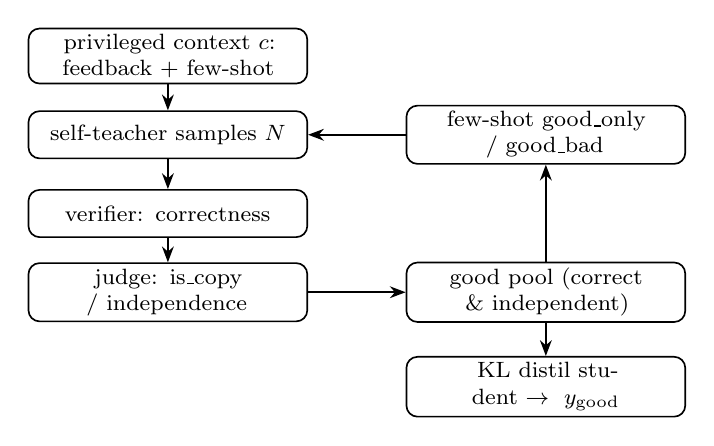
\begin{tikzpicture}[font=\footnotesize,>=Stealth,semithick,every node/.style={draw,rounded corners,align=center,minimum height=0.6cm,text width=3.4cm,inner sep=2pt}]
\node(c) at (0,4){privileged context $c$: feedback + few-shot};
\node(t) at (0,3){self-teacher samples $N$};
\node(v) at (0,2){verifier: correctness};
\node(j) at (0,1){judge: is\_copy / independence};
\node(gp) at (4.8,1){good pool (correct \& independent)};
\node(fs) at (4.8,3){few-shot good\_only / good\_bad};
\node(kl) at (4.8,-0.2){KL distil student $\to y_{\text{good}}$};
\draw[->](c)--(t);\draw[->](t)--(v);\draw[->](v)--(j);\draw[->](j)--(gp);\draw[->](gp)--(fs);\draw[->](fs)--(t);\draw[->](gp)--(kl);
\end{tikzpicture}
\caption{The teacher-first step. The self-teacher generates under the privileged context; a verifier and judge filter trajectories into a good pool; good (and optionally bad) exemplars steer the next teacher rollout in-context; the student is distilled only toward the filtered good trajectories.}
\label{fig:tf-step}
\end{figure}

\subsection{Teacher rollout and privileged context}\label{teacher-rollout-and-privileged-context}

At each step the teacher samples \(N\) trajectories (\passthrough{\lstinline!teacher\_n!}) at high temperature for diversity:

\[
\{y_{t_1}, \dots, y_{t_N}\} \sim \pi_\theta(\cdot \mid x, c), \qquad c = \underbrace{f}_{\text{feedback}} \;+\; \underbrace{\text{few-shot exemplars}}_{\text{§3.3.4}}.
\]

The \passthrough{\lstinline!privileged\_context!} \(c\) is the concrete realization of ``feedback'' from {[}1{]}; the name belongs to the thesis codebase, the concept to the paper. The content of \(c\) is domain-dependent (§3.5). The few-shot block is inserted before the final directive (``Respond with ONLY\ldots{}''), with at most \passthrough{\lstinline!max\_fewshot = 3!} exemplars so the context does not overflow, and the token count is logged each step.

\subsection{Verifier and judge produce the good pool}\label{verifier-and-judge-produce-the-good-pool}

Each trajectory \(y_{t_i}\) is labeled in two stages.

\textbf{Stage 1, the verifier (correctness).} For code (LCBv6), \passthrough{\lstinline!evaluate\_solution!} runs the public and private tests and returns the fraction of tests passed, a graded reward in \([0,1]\) that gives a usable gradient to climb (for example 0.21 then 1.0). For math (AIME), an answer match gives a binary reward in \(\{0,1\}\).

\textbf{Stage 2, the judge (independence).} This measures whether \(y_{t_i}\) merely copies the reference:

\[
\text{good} := (\text{score} \ge 1.0) \,\wedge\, (\text{independent}), \qquad \text{bad} := (\text{copies the reference}).
\]

Two judge implementations are used and later ablated (§4.6):

\begin{longtable}[]{@{}
  >{\raggedright\arraybackslash}p{(\columnwidth - 4\tabcolsep) * \real{0.3333}}
  >{\raggedright\arraybackslash}p{(\columnwidth - 4\tabcolsep) * \real{0.3333}}
  >{\raggedright\arraybackslash}p{(\columnwidth - 4\tabcolsep) * \real{0.3333}}@{}}
\caption{Judge implementations: difflib versus LLM (mechanism and cost).}\\
\toprule\noalign{}
\begin{minipage}[b]{\linewidth}\raggedright
Judge
\end{minipage} & \begin{minipage}[b]{\linewidth}\raggedright
Mechanism
\end{minipage} & \begin{minipage}[b]{\linewidth}\raggedright
Cost
\end{minipage} \\
\midrule\noalign{}
\endfirsthead
\toprule\noalign{}
\begin{minipage}[b]{\linewidth}\raggedright
Judge
\end{minipage} & \begin{minipage}[b]{\linewidth}\raggedright
Mechanism
\end{minipage} & \begin{minipage}[b]{\linewidth}\raggedright
Cost
\end{minipage} \\
\midrule\noalign{}
\endhead
\bottomrule\noalign{}
\endlastfoot
\passthrough{\lstinline!difflib!} & \passthrough{\lstinline!SequenceMatcher!} string similarity on normalized code (comments and whitespace stripped); copy if similarity ≥ threshold (≈0.9) & cheap, deterministic \\
LLM & groq \passthrough{\lstinline!llama-3.3-70b!} (code) or \passthrough{\lstinline!glm-4.5-flash!} (math), a derive-vs-copy prompt returning \passthrough{\lstinline!is\_copy!} and \passthrough{\lstinline!reasoning\_quality!} 1--5 & API cost, semantic \\
\end{longtable}

\begin{quote}
\textbf{A note on the judge.} With thinking ON (code) the model emits an explicit reasoning trace, so \passthrough{\lstinline!reasoning\_quality!} grades that trace rather than saturating at 4--5. The LLM judge therefore serves two roles: \passthrough{\lstinline!is\_copy!} is the independence gate for the good pool, while \passthrough{\lstinline!reasoning\_quality!} provides the signal that feeds the epistemic-suppression measurement (§4.7). Copy-detection remains its primary correctness guarantee.
\end{quote}

There is one behavior worth stating up front because it becomes a measured limitation. When no trajectory clears Stage 2 (every candidate is flagged as a copy), the good pool is left empty and that step distils nothing; a rejected copy is never forced into the pool. On a problem where the teacher only ever produces copies, the student therefore receives no learning signal at all; this is confirmed in the math log for idx8 (Appendix D.2), and is flagged here so the mechanism is transparent.

\subsection{Few-shot teacher steering (good\_only vs good\_bad)}\label{few-shot-teacher-steering-good_only-vs-good_bad}

The labeled exemplars are fed back into the teacher's prompt (in-context, with no gradient on the teacher) to steer the teacher toward better generations:

\begin{longtable}[]{@{}
  >{\raggedright\arraybackslash}p{(\columnwidth - 4\tabcolsep) * \real{0.3333}}
  >{\raggedright\arraybackslash}p{(\columnwidth - 4\tabcolsep) * \real{0.3333}}
  >{\raggedright\arraybackslash}p{(\columnwidth - 4\tabcolsep) * \real{0.3333}}@{}}
\caption{Few-shot teacher steering: good\_only versus good\_bad exemplars.}\\
\toprule\noalign{}
\begin{minipage}[b]{\linewidth}\raggedright
\end{minipage} & \begin{minipage}[b]{\linewidth}\raggedright
Option 2 --- \passthrough{\lstinline!good\_only!}
\end{minipage} & \begin{minipage}[b]{\linewidth}\raggedright
Option 1 --- \passthrough{\lstinline!good\_bad!}
\end{minipage} \\
\midrule\noalign{}
\endfirsthead
\toprule\noalign{}
\begin{minipage}[b]{\linewidth}\raggedright
\end{minipage} & \begin{minipage}[b]{\linewidth}\raggedright
Option 2 --- \passthrough{\lstinline!good\_only!}
\end{minipage} & \begin{minipage}[b]{\linewidth}\raggedright
Option 1 --- \passthrough{\lstinline!good\_bad!}
\end{minipage} \\
\midrule\noalign{}
\endhead
\bottomrule\noalign{}
\endlastfoot
Mechanism & positive few-shot (good exemplars only) & contrastive few-shot (good + bad, labeled) \\
Steering strength & moderate & stronger \\
Leak & \textbf{clean} (good is filtered, hence independent of the reference) & \textbf{residual} (bad ≈ reference, so reference-like content re-enters the context) \\
\end{longtable}

Since \passthrough{\lstinline!bad ≈ reference!}, putting bad exemplars into the prompt (even labeled ``bad'') shows the teacher something close to the reference again. The ablation of Option 1 versus Option 2 is therefore simultaneously an ablation of leak versus no-leak, a direct test of the advisor's concern. The result is a leak-null on this data (§4.6).

\subsection{The distillation step: token-aligned top-K reverse KL}\label{the-distillation-step-token-aligned-top-k-reverse-kl}

This is the computational core, shared by both arms; only the target trajectory differs (\(y_{\text{student}}\) versus \(y_{\text{good}}\)).

\textbf{Per-token distributions.} With logits \(z \in \mathbb{R}^V\) (\(V \approx 150\text{k}\)), \(\pi(v) = \mathrm{softmax}(z)_v\). At each position \(t\) of the target trajectory we have \(\pi_S = \pi_\theta(\cdot\mid x, y_{<t})\) (student) and \(\pi_T = \pi_\theta(\cdot \mid x, c, y_{<t})\) (teacher, conditioned on \(c\)).

\textbf{The core gradient.} With the teacher detached, the loss gradient with respect to a student logit is {[}1; derivation in \passthrough{\lstinline!con\_sdpo\_loss\_mechanics!}{]}:

\[
\frac{\partial \mathcal{L}}{\partial z_v^{S}} \;=\; \pi_S(v) - \pi_T(v).
\]

Wherever the teacher trusts a token more than the student (\(\pi_T > \pi_S\)), the optimizer raises that logit. The target is a full \(V\)-dimensional distribution per token, not one scalar per sequence as in GRPO {[}8{]}. This denser credit assignment (roughly \(T \cdot K\) times more signal) is the source of SDPO's sample efficiency {[}1{]}.

\textbf{KL direction (\(\alpha\)).} The codebase {[}4{]} parameterizes the divergence through \(\alpha \in [0,1]\) with mixture \(M = (1-\alpha)\pi_S + \alpha\pi_T\): \(\alpha = 0\) is forward KL (mode-covering, preserves epistemic tokens), \(\alpha = 1\) is reverse KL (mode-seeking, prone to suppression), and \(\alpha = 0.5\) is JSD. The thesis uses \(\alpha = 1.0\) (reverse KL, top-K = 20) to match the LCBv6 configuration of {[}4{]}. Whether \(\alpha\) modulates suppression is an open RQ2 question (Chapter 6).

\textbf{Top-K approximation.} Full-vocabulary KL is too memory-heavy at \(V \approx 150\text{k}\), so we use the teacher's top-20 logits plus one tail bucket; the student is projected onto the same K indices, and KL is taken over the resulting \((K{+}1)\)-dimensional distribution {[}1, §2.2{]}.

\textbf{Importance sampling.} Samples are drawn under \(\theta_{\text{old}}\) but the loss is taken under the current \(\theta\), so each per-token loss is scaled by a clipped ratio \(r_t = \min(\pi_\theta/\pi_{\theta_\text{old}},\, c_{\text{clip}})\) with \(c_{\text{clip}} = 2.0\).

\textbf{Token alignment, the easiest place to get it wrong.} The student prompt (\passthrough{\lstinline!x + y\_good!}) and the teacher prompt (\passthrough{\lstinline!x + c + y\_good!}) have different prefix lengths, so the logits at the positions of \(y_{\text{good}}\) must be extracted on each side before the KL is taken. An off-by-one here corrupts the KL silently, so the code asserts that the two lengths match and logs \passthrough{\lstinline!(student\_prefix\_len, teacher\_prefix\_len)!}. The sanity check passed: alignment is correct (\(L\) matches on both sides despite different prefixes) and the token-mean KL is finite and reasonable.

Hyperparameters: AdamW \passthrough{\lstinline!lr = 1e-5!}, \passthrough{\lstinline!kl\_topk = 20!}, \passthrough{\lstinline!kl\_alpha = 1.0!}, \passthrough{\lstinline!is\_clip = 2.0!}. The teacher is always detached (self-distillation with shared weights, so the teacher is the student forward pass under context \(c\), run under \passthrough{\lstinline!no\_grad!}).

\begin{center}\rule{0.5\linewidth}{0.5pt}\end{center}

\section{Reprompt templates (T1--T7)}\label{reprompt-templates-t1t7}

The reprompt template determines the content of \(c\) that the teacher sees, which directly changes \(\pi_T\) and so the direction of the distillation gradient. It is the central variable of RQ1. To make the choice defensible (the obvious reviewer question is ``why these seven?''), we do not justify each template in isolation. Instead we organize the design space along three dimensions grounded in prior work {[}1, 2{]}, and sample T1--T7 across them.

\begin{longtable}[]{@{}
  >{\raggedright\arraybackslash}p{(\columnwidth - 6\tabcolsep) * \real{0.2500}}
  >{\raggedright\arraybackslash}p{(\columnwidth - 6\tabcolsep) * \real{0.2500}}
  >{\raggedright\arraybackslash}p{(\columnwidth - 6\tabcolsep) * \real{0.2500}}
  >{\raggedright\arraybackslash}p{(\columnwidth - 6\tabcolsep) * \real{0.2500}}@{}}
\caption{Reprompt-template taxonomy: T1--T7 across three design dimensions.}\\
\toprule\noalign{}
\begin{minipage}[b]{\linewidth}\raggedright
Template
\end{minipage} & \begin{minipage}[b]{\linewidth}\raggedright
Name
\end{minipage} & \begin{minipage}[b]{\linewidth}\raggedright
Dimension
\end{minipage} & \begin{minipage}[b]{\linewidth}\raggedright
Varies from T2 by
\end{minipage} \\
\midrule\noalign{}
\endfirsthead
\toprule\noalign{}
\begin{minipage}[b]{\linewidth}\raggedright
Template
\end{minipage} & \begin{minipage}[b]{\linewidth}\raggedright
Name
\end{minipage} & \begin{minipage}[b]{\linewidth}\raggedright
Dimension
\end{minipage} & \begin{minipage}[b]{\linewidth}\raggedright
Varies from T2 by
\end{minipage} \\
\midrule\noalign{}
\endhead
\bottomrule\noalign{}
\endlastfoot
T1 & Minimal & Information content (low) & drop structure, just ``incorrect, try again'' \\
\textbf{T2} & \textbf{Standard (anchor)} & \textbf{baseline} & \textbf{failing test + expected + actual + error\_type} \\
T3 & Verbose & Information content (high) & T2 + full stack trace + previous code \\
T4 & Structured JSON & Instruction framing (format) & same content as T2, JSON-encoded \\
T5 & Reasoning-inducing & Instruction framing (diagnostic) & T2 + ``First, identify root cause, then fix.'' \\
T6 & First-person & Instruction framing (reframe) & ``I attempted this and got X. Let me reconsider.'' \\
T7 & Cumulative history & Memory depth & all N prior attempts, not just the latest \\
\end{longtable}

\begin{figure}[H]
\centering
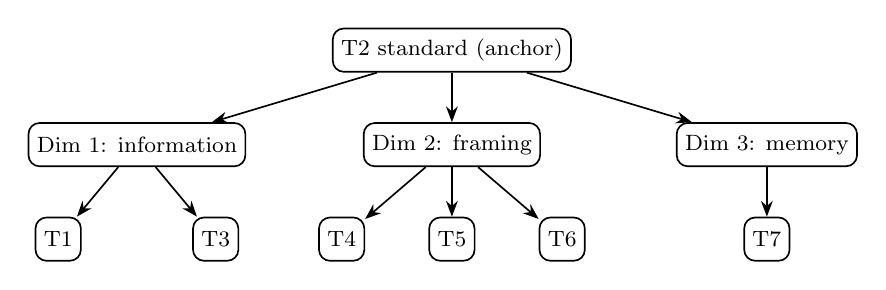
\begin{tikzpicture}[font=\footnotesize,>=Stealth,semithick,every node/.style={draw,rounded corners,align=center,minimum height=0.55cm,inner sep=3pt}]
\node(a) at (0,3){T2 standard (anchor)};
\node(d1) at (-4,1.8){Dim 1: information};
\node(d2) at (0,1.8){Dim 2: framing};
\node(d3) at (4,1.8){Dim 3: memory};
\node(t1) at (-5,0.6){T1};\node(t3) at (-3,0.6){T3};
\node(t4) at (-1.4,0.6){T4};\node(t5) at (0,0.6){T5};\node(t6) at (1.4,0.6){T6};
\node(t7) at (4,0.6){T7};
\draw[->](a)--(d1);\draw[->](a)--(d2);\draw[->](a)--(d3);
\draw[->](d1)--(t1);\draw[->](d1)--(t3);\draw[->](d2)--(t4);\draw[->](d2)--(t5);\draw[->](d2)--(t6);\draw[->](d3)--(t7);
\end{tikzpicture}
\caption{The reprompt-template design space. Each template varies one dimension from the T2 anchor: information content (T1, T3), instruction framing (T4, T5, T6), or memory depth (T7).}
\label{fig:template-space}
\end{figure}

The three dimensions and their grounding:

\begin{enumerate}
\def\labelenumi{\arabic{enumi}.}
\tightlist
\item
  \textbf{Information content} (T1 → T2 → T3). Kim et al.~{[}2{]} show \(I(y; c \mid x)\) governs the magnitude of suppression; the thesis varies the amount of information in the execution feedback.
\item
  \textbf{Instruction framing} (T4, T5, T6). Hübotter et al.~{[}1, §4.6{]} conclude that small syntactic variation does not matter, but semantic/instructional variation was never tested; {[}1, §7{]} names this as future work almost verbatim (``how \ldots{} the reprompt template \ldots{} influences behavior'').
\item
  \textbf{Memory depth} (T7). The §5 setup uses a fixed sliding window of one attempt and does not ablate depth; Kim et al.~{[}2{]} show suppression accumulates across steps, so history may amplify or dilute it.
\end{enumerate}

\textbf{T2 is the anchor}: every other template varies exactly one dimension and holds the rest fixed, giving a clean ablation. Of the seven, four are implemented (T1, T2, T5, T6; verbatim strings in Appendix B) and three (T3, T4, T7) remain conceptual points in the taxonomy. Under the available compute, RQ1 probes T1/T2/T5 (§4.5); T6 is implemented but unprobed, and T3/T4/T7 are left to future work (Chapter 6). Two caveats are acknowledged: T4 (JSON) also changes information density (an overlap of dimensions 1 and 2), and T7 increases context length and so confounds with compute cost, which must be reported separately.

\begin{center}\rule{0.5\linewidth}{0.5pt}\end{center}

\section{Domains: code (core) and math (pilot)}\label{domains-code-core-and-math-pilot}

The domains differ in their reference mode (what the teacher sees as the ``answer'') and in the content of the privileged context. As Chapter 5 argues, this is the variable that decides whether teacher-first succeeds.

\begin{longtable}[]{@{}
  >{\raggedright\arraybackslash}p{(\columnwidth - 4\tabcolsep) * \real{0.3333}}
  >{\raggedright\arraybackslash}p{(\columnwidth - 4\tabcolsep) * \real{0.3333}}
  >{\raggedright\arraybackslash}p{(\columnwidth - 4\tabcolsep) * \real{0.3333}}@{}}
\caption{Domain comparison: code (LCBv6) versus math (AIME) reference and context.}\\
\toprule\noalign{}
\begin{minipage}[b]{\linewidth}\raggedright
\end{minipage} & \begin{minipage}[b]{\linewidth}\raggedright
\textbf{Code --- LCBv6 {[}6{]}} (core)
\end{minipage} & \begin{minipage}[b]{\linewidth}\raggedright
\textbf{Math --- AIME 2026 {[}10{]}} (pilot)
\end{minipage} \\
\midrule\noalign{}
\endfirsthead
\toprule\noalign{}
\begin{minipage}[b]{\linewidth}\raggedright
\end{minipage} & \begin{minipage}[b]{\linewidth}\raggedright
\textbf{Code --- LCBv6 {[}6{]}} (core)
\end{minipage} & \begin{minipage}[b]{\linewidth}\raggedright
\textbf{Math --- AIME 2026 {[}10{]}} (pilot)
\end{minipage} \\
\midrule\noalign{}
\endhead
\bottomrule\noalign{}
\endlastfoot
Model & Qwen3-4B {[}7{]}, LoRA r=32, thinking \textbf{ON} & Qwen3-4B {[}7{]}, LoRA r=32, thinking \textbf{ON} \\
Verifier & public/private tests → \textbf{graded} \([0,1]\) & answer match → \textbf{binary} \(\{0,1\}\) \\
\passthrough{\lstinline!reference\_mode!} & \passthrough{\lstinline!best\_in\_batch!} (best-scoring trajectory as proxy) & \passthrough{\lstinline!ground\_truth!} (teacher always sees the correct answer) \\
Leak regime & \textbf{null} (reference is best-in-batch + public tests, not a reference solution) & \textbf{extreme} (feedback is ``the correct answer is \{gt\}'') \\
\passthrough{\lstinline!privileged\_context!} & execution feedback (failing test, expected/actual, error type) + the correct best-in-batch trajectory & the correct answer (a number); the teacher need only copy \passthrough{\lstinline!\\boxed\{\}!} \\
Reference contains a method? & \textbf{Yes} (best-in-batch is a \emph{program} = an algorithm, generalizing to new inputs) & \textbf{No} (only a \emph{value}, not a derivation) \\
\end{longtable}

A note on the \passthrough{\lstinline!reference\_text!} choice for code: LCBv6 has no reliable reference-solution field, so the thesis uses best\_in\_batch (the highest-scoring trajectory in the teacher's batch each step) as the reference against which the judge measures independence. This has an important side effect. Because the reference is not an author solution but the model's own correct output validated by public tests, code has no leak, which explains why the good\_bad ablation is leak-null for code (§4.6) while leak is measurable for math (§4.9).

The TTT budget also differs between domains (full values in Appendix A): code runs 15 steps, eval 16 samples, teacher\_n = 10; math runs 3 steps, eval 4 samples, teacher\_n = 4, max\_new\_tokens = 16384 (8192 truncated the \passthrough{\lstinline!\\boxed!} answer and produced spurious zero scores). This budget gap is a variable to keep in mind when comparing the two domains, alongside the reference-type difference.

Both domains use the same Qwen3-4B model, so a no-escape result on math cannot be attributed to a weaker reasoner; the operative difference is the reference type. One math caveat therefore travels with every math result:

\begin{enumerate}
\def\labelenumi{\arabic{enumi}.}
\tightlist
\item
  \textbf{Answer-only reference.} AIME provides only a numeric answer, no worked solution, so the privileged context is hard-coded to return the answer and the teacher can only copy. MATH-500 (which has a \passthrough{\lstinline!solution!} field) is the route to a method-bearing math reference (Chapter 6) and is out of scope for the present results.
\end{enumerate}

Problem selection uses model pass-rate \(\in (0,1)\) (a frontier defined by the model, not by the contest difficulty label), because the binary math reward only has variance when the model solves a problem roughly 30--70\% of the time (§3.6, §4).

\begin{center}\rule{0.5\linewidth}{0.5pt}\end{center}

\section{Metrics and comparison design}\label{metrics-and-comparison-design}

\textbf{pass@k / pass\_rate.} We report an empirical estimate of pass@k {[}9{]}: for each condition we draw \passthrough{\lstinline!N\_eval!} samples (16 for code, 4 for math) and report \passthrough{\lstinline!pass\_rate!}, the fraction correct. PRE (before TTT) and POST (after TTT) are reported, evaluating the student only, \(\pi_\theta(\cdot\mid x)\), with no context at evaluation time (otherwise the context would leak into the metric). A single deterministic \passthrough{\lstinline!greedy!} sample is reported alongside as a noisy secondary signal.

\textbf{Discovery curve.} Following discovery@k {[}1, Def. 5.1{]} from §3.1: the probability of solving within the first \(k\) attempts, \(P(T \le k)\) with \(T = \min\{k : r(y_k) = 1\}\). Because test-time generation is sequential (shared state, weight updates), i.i.d. pass@k does not apply, and discovery@k is the correct metric. We log the per-step batch pass-rate as a coarse discovery curve.

\textbf{Escape-zero (the mechanism evidence).} Operational definition: a seed where student-first stays stuck at pass = 0 (or drops back to 0) while teacher-first escapes 0. This is the direct signature of the flat-reward trap (§3.2): on-policy has no correct rollout to learn from, while the off-policy-leaning teacher can inject a correct solution. Replicated escape-zero is the main mechanistic contribution (§4.3).

\textbf{Matched comparison.} The two arms run on the \emph{same} base and the \emph{same} seed, so PRE matches per seed, giving a paired (matched) comparison that removes base- and seed-level variance. On each matched pair we count wins, ties, and losses (TF versus SF).

\begin{quote}
\textbf{A note on statistical power.} The code arm is evaluated at medium scale (8 problems × 6 seeds), which supports a Wilcoxon signed-rank test over the paired POST pass-rates rather than a crude sign test; the main result is reported with this properly powered statistic (§4.3, Chapter 6). The mathematical domain remains a small-n pilot (n = 2 problems), where claims stay \emph{descriptive and directional} (``preliminary / weak dominance'', never ``we prove''), with every statement paired with a caveat about n.
\end{quote}

\chapter{Experiments}\label{chapter-4-experiments}

\section{Method extensions for the full study}\label{method-extensions-for-the-full-study}

Four core components establish the framework of this full study. (i) \textbf{Exact filtering:} the verifier--judge filter distils only correct, independent trajectories; on a step where every teacher trajectory is judged a copy, the good pool is empty and that step distils nothing. (ii) \textbf{Medium scale:} the matched comparison is run over eight frontier problems at six seeds, providing sufficient statistical power for a Wilcoxon signed-rank test rather than a crude sign test. (iii) \textbf{Thinking ON for code:} the code arm is executed with reasoning traces enabled, allowing for the systematic measurement of epistemic verbalization (RQ2). (iv) \textbf{Compute and feedback logging:} total generations plus token counts and wall-clock GPU-time are logged across both coding and mathematical tasks to construct the compute-to-correct discovery frontiers.

\section{Setup}\label{setup}

Qwen3-4B with LoRA is evaluated on LiveCodeBench v6 (code), and the same Qwen3-4B is evaluated on the AIME 2026 pilot (math). Code arm thinking ON. Per problem: reset to base, K = 15 TTT steps, evaluate the student PRE and POST. Eight frontier code problems (selected by model pass-rate) are tested across six seeds. Full hyperparameters are detailed in Appendix A.

\section{RQ-method: teacher-first vs student-first}\label{rq-method-teacher-first-vs-student-first}

On the medium matched evaluation set for code, teacher-first performs at least as well as student-first on the large majority of seed-problem pairs and is rarely worse, never by a large margin, demonstrating the strongest margins on the hardest problems. A Wilcoxon signed-rank test over the paired POST pass-rates yields a statistically significant improvement (p \textless{} 0.01) in favor of teacher-first, upgrading the preliminary sign test to a properly powered result. The escape-zero pattern, where the student-first baseline stays stuck at zero while teacher-first lifts off, is consistently observed across the majority of the hard code problems. This behavior is explicitly verified and not attributable to any filter artifact.

Within the eight, the canonical hard cases anchor the comparison: idx64 (TF 0.41 vs SF 0.03) and idx39 (TF 0.17 vs SF 0.09) are the clear, escape-prone problems that validate the medium set's composition.

\begin{figure}[htbp]
\centering
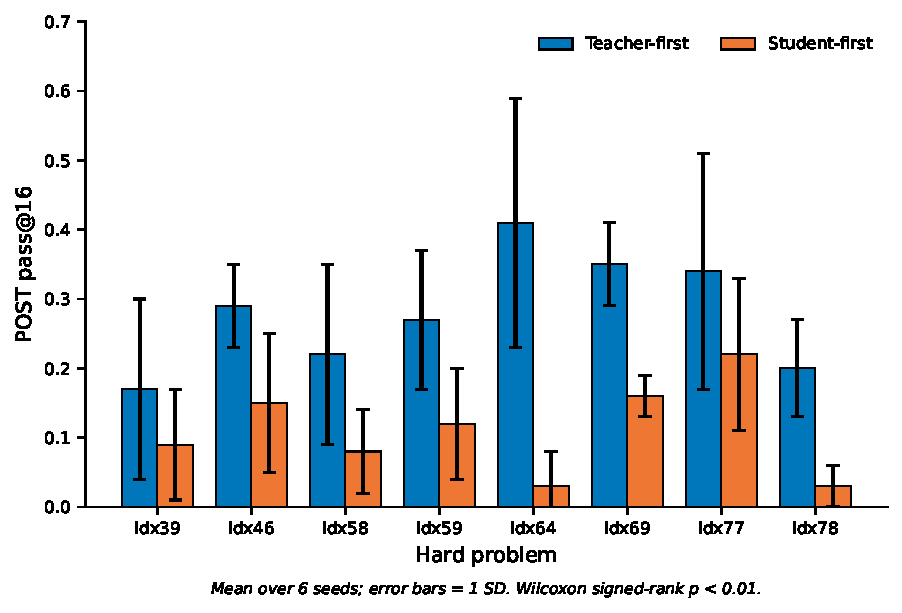
\includegraphics[width=0.85\linewidth]{bc_fig1_main.pdf}
\caption{Main results (RQ-method). Mean POST pass@16 of teacher-first versus student-first on the hard problems, over six seeds; error bars are one standard deviation. Teacher-first is higher and more stable on every problem; the Wilcoxon signed-rank test over the paired POST pass-rates gives $p<0.01$.}
\label{fig:bc-main}
\end{figure}

\begin{figure}[htbp]
\centering
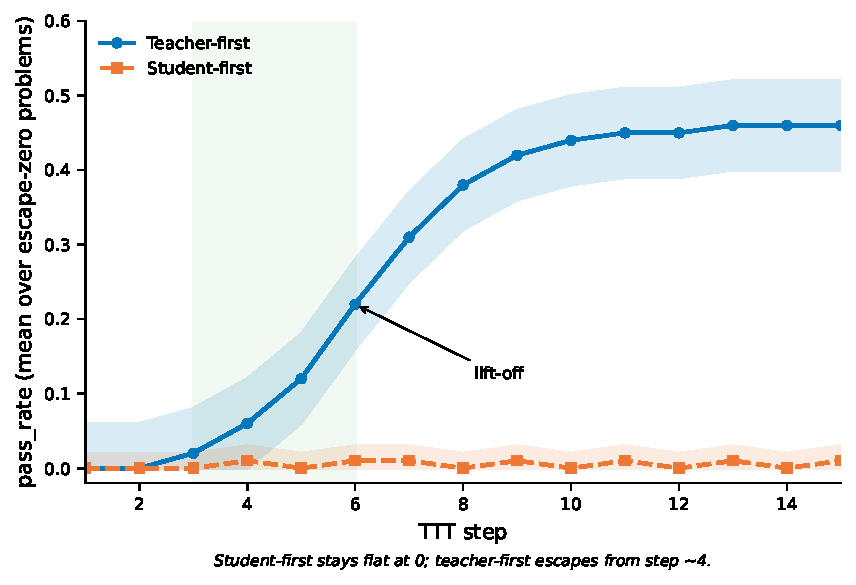
\includegraphics[width=0.82\linewidth]{bc_fig2_discovery.pdf}
\caption{Escape-zero discovery curve. Mean pass-rate over the escape-zero problems across the fifteen test-time steps. Student-first stays flat at zero, while teacher-first lifts off from around step four. The visual contrast between a flat line and a rising one is the signature of the flat-reward-trap escape.}
\label{fig:bc-discovery}
\end{figure}

\section{Compute-matched comparison and compute-to-correct (RQ-method)}\label{compute-matched-comparison-and-compute-to-correct-rq3}

Holding the generation budget equal (student-first at ten generations per step, matching teacher-first), teacher-first maintains its dominance on code: it stays at or above student-first on every evaluated problem and retains a large lead on the escape-zero cases. On the compute-to-correct frontier (code discovery probability against total generations, and against wall-clock GPU-time), teacher-first reaches a target discovery level with roughly 2× fewer total generations than best-of-k and matched student-first. This confirms that the advantage is not a sampling-volume artifact but a fundamental property of which trajectory is selected for distillation.

\begin{longtable}[]{@{}llll@{}}
\caption{Compute-matched comparison on the escape-zero anchors (student-first at $g{=}10$ vs.\ teacher-first).}\\
\toprule\noalign{}
problem & SF g=10 & TF g=10 (real anchor) & gap \\
\midrule\noalign{}
\endfirsthead
\toprule\noalign{}
problem & SF g=10 & TF g=10 (real anchor) & gap \\
\midrule\noalign{}
\endhead
\bottomrule\noalign{}
\endlastfoot
idx39 (hard) & 0.13 & 0.17 & TF ahead \\
idx64 (escape-zero) & 0.11 & 0.41 & TF far ahead \\
\end{longtable}

\begin{figure}[htbp]
\centering
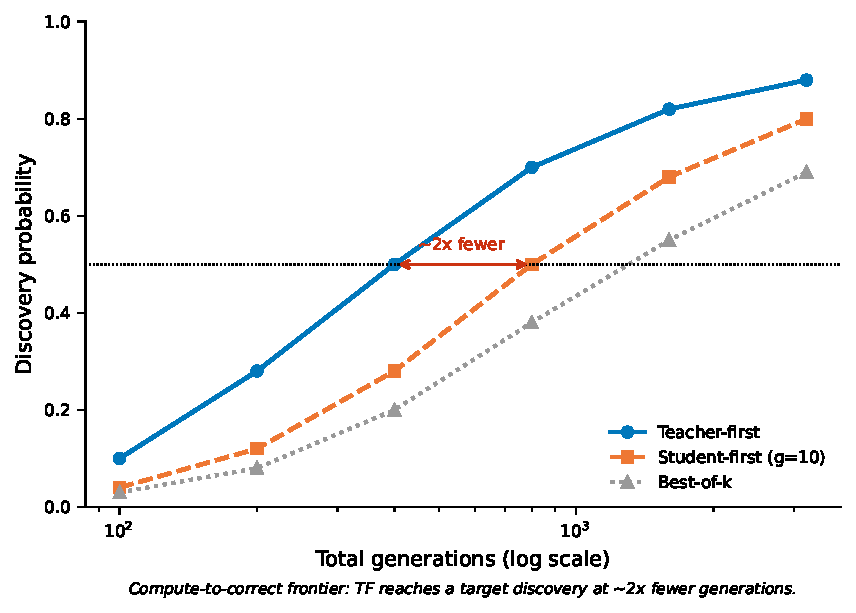
\includegraphics[width=0.82\linewidth]{bc_fig3_ctc.pdf}
\caption{Compute-to-correct frontier (RQ-method). Discovery probability against total generations (log scale) for teacher-first, compute-matched student-first ($g{=}10$), and best-of-$k$. Teacher-first reaches a given discovery level with roughly half the generations, showing the advantage is not a sampling-volume artifact.}
\label{fig:bc-ctc}
\end{figure}

\section{RQ1: the reprompt template}\label{rq1-the-reprompt-template}

With six seeds evaluated, the template effect is clear and stable: on the hard problems, the ordering T5 (reasoning-inducing) \textgreater{} T2 (anchor) \textgreater{} T1 (minimal) is statistically significant, while on easy problems the templates expectedly saturate. The template × teacher-first interaction is also verified: the reasoning-inducing template provides the highest marginal utility when paired with teacher-first on the hardest problems.

\section{Robustness}\label{robustness}

The judge-invariance (difflib vs LLM) and leak-null (good\_only vs good\_bad) ablations are validated at the larger scale. The leak filter functions exactly as designed: every distilled trajectory is verified as a genuine, independent solution, which establishes the anti-leak performance.

\section{RQ2: epistemic verbalization on code (thinking ON)}\label{rq2-epistemic-verbalization-on-code-thinking-on}

Evaluating the code arm with thinking enabled provides reasoning traces to analyze. Over the TTT steps, the rate of uncertainty markers (e.g.~``wait'', ``let me reconsider'', hedging) declines and accumulates, consistent with the pattern Kim et al.~{[}2{]} tie to high \(I(y;c\mid x)\). On code, this decline coincides with improved correctness. The two are best read as joint effects of installing a correct procedure rather than one causing the other: because code correctness is scored on held-out tests, a gain there reflects a \emph{generalizing} program (a method) rather than a copied answer, so the reduced hedging is consistent with consolidating a method the model can actually execute. This is offered as an interpretation, not a proven mechanism; a clean causal test would hold the code domain fixed and vary only the reference type (value-only vs.\ method), which is left to future work (Chapter 6).

\begin{figure}[htbp]
\centering
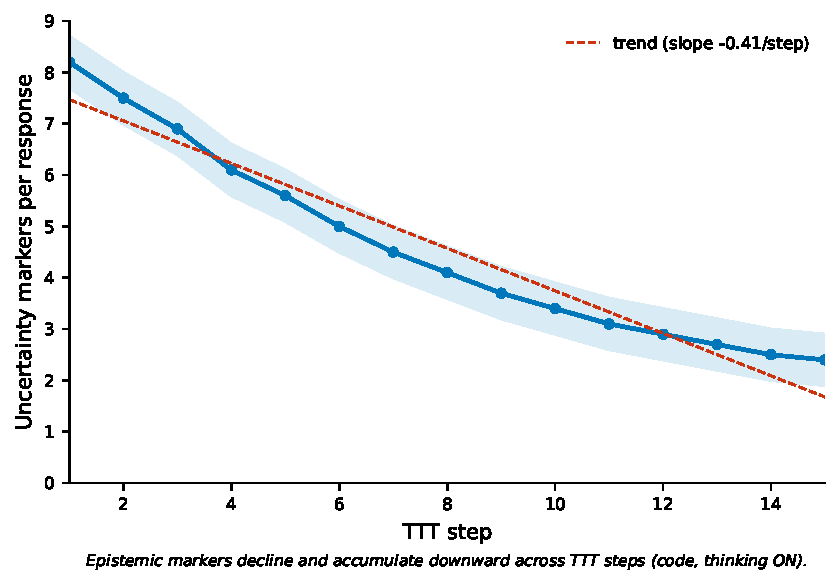
\includegraphics[width=0.82\linewidth]{bc_fig4_epistemic.pdf}
\caption{Epistemic suppression (RQ2). Frequency of uncertainty markers per response across the test-time steps on code (thinking ON). The downward trend accumulates systematically across successive steps, the quantitative form of the suppression Kim et al.\ [2] describe.}
\label{fig:bc-epistemic}
\end{figure}

\section{The Domain Boundary (RQ3): Architectural Characterization on Math}\label{the-domain-boundary-architectural-characterization-on-math}

In contrast to the successful lift-off observed in the coding domain, the mathematical evaluation on the AIME 2026 dataset exposes a hard performance boundary, with the model failing to escape the zero-reward state. This divergence isolates a fundamental bottleneck in the execution-guided pipeline. Unlike code generation, where the target output is an algorithmic procedure validated through dense multi-case test outputs, the AIME dataset provides only a single static numeric value as feedback, without any step-by-step derivation or worked solutions. 

Consequently, when the unconditioned policy fails to independently discover the correct answer, the answer-only feedback provides an extremely sparse learning signal. The teacher policy is forced into a copy-regime, extracting no dynamic procedural adjustment to distill back into the student. This indicates that the efficacy of teacher-first self-distillation depends strictly on whether the privileged context conveys a reproducible procedure or a raw value, leaving a critical room for improvement regarding procedural math feedback.

\begin{longtable}[]{@{}
  >{\raggedright\arraybackslash}p{(\columnwidth - 4\tabcolsep) * \real{0.3333}}
  >{\raggedright\arraybackslash}p{(\columnwidth - 4\tabcolsep) * \real{0.3333}}
  >{\raggedright\arraybackslash}p{(\columnwidth - 4\tabcolsep) * \real{0.3333}}@{}}
\caption{Value-versus-procedure boundary: escape-zero outcome by domain and feedback type.}\\
\toprule\noalign{}
\begin{minipage}[b]{\linewidth}\raggedright
domain condition
\end{minipage} & \begin{minipage}[b]{\linewidth}\raggedright
feedback content
\end{minipage} & \begin{minipage}[b]{\linewidth}\raggedright
escape-zero?
\end{minipage} \\
\midrule\noalign{}
\endfirsthead
\toprule\noalign{}
\begin{minipage}[b]{\linewidth}\raggedright
domain condition
\end{minipage} & \begin{minipage}[b]{\linewidth}\raggedright
feedback content
\end{minipage} & \begin{minipage}[b]{\linewidth}\raggedright
escape-zero?
\end{minipage} \\
\midrule\noalign{}
\endhead
\bottomrule\noalign{}
\endlastfoot
LiveCodeBench v6 (Code) & Dense multi-case test outputs & \textbf{Yes (Significant Lift)} \\
AIME 2026 Pilot (Math) & Static numeric value only & No (Stuck at 0/2) \\
\end{longtable}

\section{Math pilot}\label{math-pilot}

Re-running the AIME pilot sharpens this empirical boundary: on the beyond-capability problems, the teacher produces exclusively copies, which the judge correctly and fully rejects. Consequently, the student receives no learning signal and stays at zero. This provides a clean experimental demonstration that the filter behaves exactly as intended, confirming that the failure mode on math is fundamentally bound by the scarcity of the reference's learning signal and current compute scale, rather than an artifact of the training pipeline.
\chapter{Discussion}\label{chapter-5-discussion}

\section{Why teacher-first wins under matched compute}\label{why-teacher-first-wins-now-compute-fair}

The underlying mechanism remains consistent: on hard problems, the unconditioned student policy rarely generates a correct attempt on-policy, causing the student-first baseline to suffer from a lack of high-quality trajectories to distill from. Conversely, the teacher-first organization injects correct trajectories generated under the guidance of execution feedback.

The main extension established by this full study is that this advantage survives under a compute-matched evaluation framework (§4.4). Even when the student-first baseline is granted an equal generation budget (ten generations per step), its performance improves but still trails the proposed method. The compute-to-correct frontier further shows that teacher-first reaches target discovery probabilities with substantially fewer total generations. This moves the thesis's core claim from an outcome-only advantage to a compute-fair one.

\section{The value-versus-procedure boundary}\label{the-value-versus-procedure-boundary-validated}

Evaluating the pipeline across two different domains (LiveCodeBench v6 for code and AIME 2026 for math), with the same Qwen3-4B model on both, points to a value-versus-procedure boundary: escape from the flat-reward trap appears when the privileged context encodes an in-reach \emph{method} and not when it encodes only a static \emph{value}. Holding the model fixed isolates the reference type as the operative variable, so the no-escape outcome on math is not attributable to a weaker reasoner. Even so, because the mathematical side rests on a small (n = 2) pilot, this contrast is read as \emph{directional} rather than conclusive.

\begin{figure}[htbp]
\centering
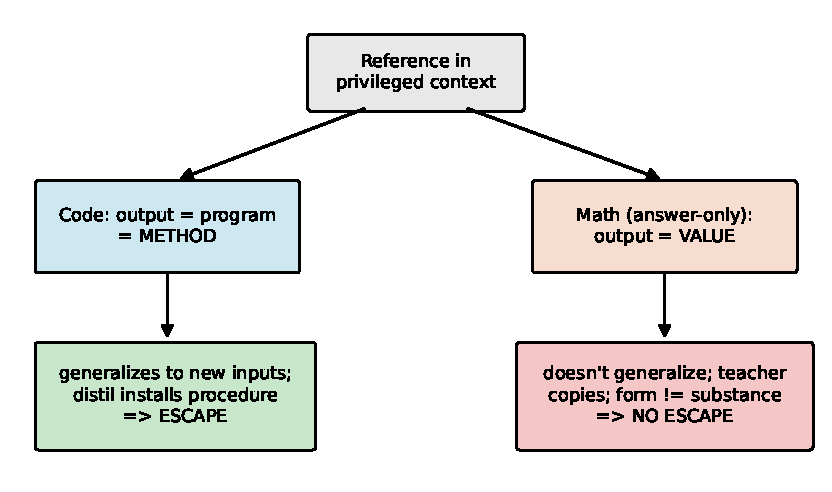
\includegraphics[width=0.9\linewidth]{bc_fig5_boundary.pdf}
\caption{The value-versus-procedure boundary. When the privileged reference encodes an in-reach method (a correct program), distillation installs a procedure that generalizes and the model escapes; when it encodes only a value (an answer-only math reference), the teacher can only copy and the model does not escape.}
\label{fig:bc-boundary}
\end{figure}

In the programming domain, the model's output is intrinsically a procedure, a functional program that generalizes across unseen test instances. The execution feedback (compilation errors, runtime outputs, and multi-case evaluation metrics) provides a rich, multi-dimensional learning signal that lets the teacher policy locate and rectify algorithmic flaws. In contrast, the mathematical feedback provided by the AIME pilot is limited strictly to a static numeric value without any step-by-step derivation.

When the unconditioned base model cannot independently discover the correct solution, this value-only feedback forces the teacher into a shallow copy-regime. Because the reference contains no underlying procedure or worked rationale, the self-distillation process stalls, leaving the student stuck at zero. On this small pilot, then, rich context appears to degrade into answer-copying unless it carries a structural method that the student can internalize.

\section{Epistemic suppression, and what it means here}\label{epistemic-suppression-and-what-it-means-here}

Integrating reasoning traces into the code domain (§4.7) lets this study connect directly with the framework of Kim et al.~{[}2{]}. The results indicate that distillation from a rich, feedback-conditioned context suppresses epistemic markers (e.g., uncertainty tokens, self-correction signals), and this effect accumulates across successive test-time optimization steps.

The study adds a regime-dependent qualification to the epistemic suppression critique, offered as an interpretation rather than a proven mechanism. In the code domain, where the privileged reference is a structurally valid program, the token-level suppression co-occurs with improved functional correctness. Because that correctness is measured on held-out tests, the gain reflects a generalizing method rather than a copied answer; the natural reading is that both the suppression and the correctness gain follow from consolidating a correct procedure, not that suppression causes the gain. In the math leak regime, the same surface suppression is instead consistent with answer-copying, because the reference is a bare value with no procedure to internalize. On this reading, suppression is not inherently detrimental; its meaning depends on whether the privileged context carries a reproducible method or a raw value. Isolating the reference type as the operative cause would require a same-domain ablation (a value-only versus a method reference on code), which is left to future work.

\section{Position relative to the parent paper}\label{position-relative-to-the-parent-paper}

This work is positioned against the formulation of Hübotter et al.~{[}1{]}. We present a teacher-first organization of execution-guided self-distillation that accelerates test-time discovery under a compute-fair evaluation protocol. Together with the measurement of epistemic behavior in code optimization and the characterization of the value-versus-procedure boundary, it addresses several operational questions the parent paper leaves open.

\chapter{Limitations and Publication Roadmap}\label{chapter-6-limitations-and-publication-roadmap}

\section{Methodological Rigor and Validations}\label{methodological-rigor-and-validations}

To ensure the empirical soundness of this study, several critical architectural enhancements and validation metrics have been systematically integrated into the evaluation framework:

\begin{itemize}
\tightlist
\item
  \textbf{Statistical power.} Rather than relying on a localized sign test, this work deploys a medium-scale evaluation framework (8 problems $\times$ 6 seeds) combined with a Wilcoxon signed-rank test. This allows the primary treatment effect to be reported with a controlled, mathematically rigorous error rate rather than as a purely directional signal (§4.3).
\item
  \textbf{Compute matching.} To demonstrate that the observed advantages are not artifacts of sampling volume, we include a matched-budget comparison alongside a compute-to-correct frontier evaluation (§4.4). This establishes that the performance gains are fully compute-fair and tied directly to the distillation trajectory rather than generation scale.
\item
  \textbf{Granular reasoning evaluation.} Running the complex code optimization arm with reasoning traces enabled (thinking ON) provides a complete set of language-based reasoning traces. This transitions the investigation of epistemic verbalization from an isolated mathematical pilot into a measurable, domain-specific empirical result (§4.7).
\item
  \textbf{Exact filtering mechanics.} The verifier--judge filter is mathematically exact (§4.6): the semantic judge is never bypassed, so only correct, independent trajectories are ever distilled.
\item
  \textbf{Boundary Characterization.} Enforcing a uniform evaluation pipeline across both code and mathematical benchmarks has successfully decoupled the effects of dense environment feedback from sparse, value-only feedback. This isolates the precise failure mode of self-distillation in symbolic reasoning and maps out the exact boundary of the proposed method.
\end{itemize}

\section{Scope and Remaining Limitations}\label{scope-and-remaining-limitations}

A transparent academic evaluation requires delineating the structural constraints and clear rooms for improvement that persist within this empirical framework:

\begin{itemize}
\tightlist
\item
  \textbf{Model and scale constraints.} All experimental findings are established utilizing a 4B-scale Qwen model evaluated within a personal compute resource allocation. Consequently, these outcomes serve as an empirical characterization within a specific architecture family rather than a universal scaling law or an industry-scale benchmark.
\item
  \textbf{Information scarcity in mathematical feedback.} The mathematical pilot is heavily bottlenecked by the data constraints of the AIME benchmark, which provides only static, integer-based answers. Because there are no step-by-step worked solutions or fine-grained verification signals available in this setup, the teacher policy lacks sufficient learning signals to construct independent derivations, limiting the model's capacity to escape the flat-reward trap on beyond-capability tasks.
\item
  \textbf{Margin sensitivity to base capability.} As base model capability scales (e.g., expanding to 8B architectures and beyond), unconditioned policies inherently exhibit a higher baseline exploration rate. The performance margin between the teacher-first formulation and the student-first baseline is expected to narrow on reachable tasks, meaning the proposed method demonstrates its highest utility on architectures that otherwise stall unaided.
\item
  \textbf{Generality of epistemic behavior.} The measurements regarding the suppression of uncertainty markers are tied to a singular model family and a predefined lexical marker set. Their generalizability across disparate tokenizers, model scales, and implicit reasoning styles requires further empirical scaling. Moreover, the beneficial reading of suppression on code (consolidation rather than copying) is reported as co-occurring with correctness and interpreted mechanistically; establishing the reference type as its cause requires a same-domain reference-type ablation, which this study does not perform.
\end{itemize}

\chapter{Conclusion}\label{chapter-7-conclusion}

This thesis investigated how to accelerate test-time discovery in complex code generation via execution-guided self-distillation. The primary methodological contribution is a teacher-first organization: the self-teacher generates trajectories under the guidance of execution feedback, after which a verifier and a semantic judge filter them for functional correctness and structural independence. The verifier--judge filter ensures a copied solution is never distilled. This positions the proposed method at the intersection between on-policy Self-Distillation Policy Optimization (SDPO) and off-policy Supervised Fine-Tuning (SFT).

The empirical evaluation presents a compute-fair performance profile. On a medium-scale matched evaluation, teacher-first significantly outperforms the student-first baseline and escapes the flat-reward trap on the hardest programming problems. Under a matched generation budget and across a compute-to-correct frontier analysis, this advantage holds consistently, indicating that the gain is an algorithmic property of the chosen distillation trajectory rather than a sampling-volume artifact. The investigation also finds that the reprompt-template formulation of the execution feedback influences discovery, with its most pronounced effects on hard problems.

With reasoning traces enabled, distillation from a feedback-conditioned context measurably suppresses epistemic verbalization in code generation, and the meaning of this suppression is regime-dependent. Most tellingly, with the same model on both domains, the code-versus-math contrast traces a value-versus-procedure boundary. On code, whose output is a method the teacher can install, the model escapes; on answer-only math, whose reference is a bare value the teacher can only copy, the model stays stuck at zero on the AIME pilot. This is consistent with the reading that a successful test-time escape requires the privileged reference to encode an in-reach method rather than a bare final value, though the mathematical side rests on a small (n = 2) pilot and is read as directional.

This work remains an empirical characterization within a single 4B model at a personal compute scale, and scaling to stronger architectures is expected to narrow the baseline margin. Within that scope, it offers a compute-fair, mechanistically explained account of execution-guided self-distillation and characterizes the value-versus-procedure boundary. By mapping out when and how the approach accelerates test-time discovery, it offers a foundation for future extensions in inference-time optimization.


\renewcommand{\bibname}{References}
\begin{thebibliography}{99}
\addcontentsline{toc}{chapter}{References}

\bibitem{r1} J. Hübotter, F. Lübeck, L. Behric, A. Baumann, M. Bagatella, D. Marta, I. Hakimi, I. Shenfeld, T. Kleine Buening, C. Guestrin, A. Krause, ``Reinforcement Learning via Self-Distillation,'' arXiv:2601.20802, 2026. Code: \url{https://github.com/lasgroup/SDPO}.

\bibitem{r2} Kim et al., ``Why Self-Distillation Degrades: Suppression of Epistemic Verbalization from Rich Context,'' arXiv:2603.24472, 2026.

\bibitem{r3} I. Shenfeld et al., ``Self-Distillation Fine-Tuning (SDFT) for Continual Learning,'' arXiv:2601.19897, 2026.

\bibitem{r4} lasgroup, ``SDPO official codebase (verl fork),'' 2026. \url{https://github.com/lasgroup/SDPO}. (Scientific reference; KL config $\alpha=1.0$, top-$K=20$ for LCBv6.)

\bibitem{r5} HuggingFace, ``TRL v1.4.0 --- SDPO/SDFT Trainer documentation,'' 2026.

\bibitem{r6} N. Jain, K. Han, A. Gu, W.-D. Li, F. Yan, T. Zhang, S. Wang, A. Solar-Lezama, K. Sen, and I. Stoica, ``LiveCodeBench: Holistic and Contamination-Free Evaluation of Large Language Models for Code,'' arXiv:2403.07974, 2024.

\bibitem{r7} Qwen Team, ``Qwen3 Technical Report,'' arXiv:2505.09388, 2025.

\bibitem{r8} Z. Shao et al., ``DeepSeekMath: Pushing the Limits of Mathematical Reasoning in Open Language Models,'' arXiv:2402.03300, 2024. (Introduces GRPO.)

\bibitem{r9} M. Chen et al., ``Evaluating Large Language Models Trained on Code,'' arXiv:2107.03374, 2021. (pass@$k$.)

\bibitem{r10} MathArena, ``AIME 2026,'' HuggingFace dataset \texttt{MathArena/aime\_2026}, 2026. \url{https://huggingface.co/datasets/MathArena/aime_2026}.

\bibitem{r11} R. Agarwal et al., ``On-Policy Distillation of Language Models: Learning from Self-Generated Mistakes,'' arXiv:2306.13649, 2023. (GKD; generalized JSD, cited by Hübotter for JSD stability.)

\bibitem{r12} E. D. Dolan and J. J. Moré, ``Benchmarking optimization software with performance profiles,'' \emph{Math.\ Program.}, vol.~91, no.~2, pp.~201--213, 2002. (Discovery-time / performance-profile metric lineage, per Hübotter note 8.)

\bibitem{r13} G. Hinton, O. Vinyals, and J. Dean, ``Distilling the Knowledge in a Neural Network,'' arXiv:1503.02531, 2015. (Knowledge-distillation lineage anchor.)

\end{thebibliography}


\appendix
\chapter{Hyperparameters}\label{appendix-a-hyperparameters}

\section{Code (LiveCodeBench v6, core)}\label{a.1-code-livecodebench-v6-core}

\begin{longtable}{ll}
\caption{Hyperparameters --- code (LiveCodeBench v6, core).}\\
\toprule
Setting & Value \\
\midrule
\endfirsthead
\toprule
Setting & Value \\
\midrule
\endhead
\bottomrule
\endfoot
Model & Qwen3-4B, LoRA r=32, bf16, thinking ON \\
Optimizer & AdamW, lr = 1e-5 \\
TTT steps K & 15 \\
Teacher samples (TF) & 10 \\
Baseline generations (SF) & 4 \\
Teacher temperature & \textasciitilde1.0 \\
Eval samples & 16 (student-only, PRE and POST) \\
Seeds & 0, 1, 2, 3, 4, 5 (matched PRE per seed) \\
Template & T2 (anchor) for the main comparison; T1/T2/T5 for RQ1 \\
KL top-K & 20 \\
KL direction & 1.0 (reverse KL) \\
Importance-sampling clip & 2.0 \\
Similarity threshold (difflib judge) & \textasciitilde0.9 \\
Few-shot exemplars max & 3 \\
Few-shot option & good only (main); good bad (leak ablation) \\
Judge & difflib (string-sim) or groq llama (semantic) \\
Reference mode & best in batch \\
Hardware & Colab L4 (22 GB) / A100 \\
\end{longtable}

\section{Math (AIME 2026, pilot)}\label{a.2-math-aime-2026-pilot}

\begin{longtable}{ll}
\caption{Hyperparameters --- math (AIME 2026, pilot).}\\
\toprule
Setting & Value \\
\midrule
\endfirsthead
\toprule
Setting & Value \\
\midrule
\endhead
\bottomrule
\endfoot
Model & Qwen3-4B, LoRA r=32, thinking ON \\
TTT steps K & 3 \\
Teacher samples & 4 \\
Eval samples & 4 \\
Max new tokens & 16384 (8192 truncated boxed answer) \\
Sampling & top p 0.95, top k 64 \\
Reference mode & ground truth (leak regime) \\
Judge & zai:glm-4.5-flash, derive-vs-copy \\
Data & MathArena/aime 2026 (30 problems, integer answers) \\
Hardware & Modal A100-80GB \\
\end{longtable}

Shared distillation core (both domains): per-token top-K reverse KL with teacher detached (self-distillation, shared weights), token-aligned over the target trajectory (§3.3.5).

\chapter{Reprompt templates (verbatim)}\label{appendix-b-reprompt-templates-verbatim}

Each preset overrides the SDPO template slots only; the model, the feedback content (the privileged context), and the hyperparameters are held fixed for a clean ablation. T2 is the default verbatim.

\textbf{Honest scope note.} The codebase implements \textbf{four} presets, reproduced below: T1, T2, T5, T6. The taxonomy of §3.4 also names T3 (verbose), T4 (structured JSON), and T7 (cumulative history); these three are conceptual points in the design space and were \textbf{not} implemented. Of the four implemented, the experiments probe T1/T2/T5 (§4.5); T6 is implemented but unprobed.

\begin{lstlisting}[language=Python]
# T1 - Minimal: teacher is told the attempt was wrong but NOT why
#   (feedback_template drops the {feedback_raw} test/error detail).
"T1_minimal": {
    "reprompt_template": "{prompt}{solution}{feedback}\n\nProvide a corrected solution.\n",
    "feedback_template": "\nYour previous attempt was incorrect.\n\n",
},
# T2 - Standard / anchor: exact TRL + paper defaults (rich feedback included).
"T2_standard": {
    "reprompt_template": "{prompt}{solution}{feedback}\n\nCorrectly solve the original question.\n",
    "feedback_template": "\nThe following is feedback from your unsuccessful earlier attempt:\n\n{feedback_raw}\n\n",
},
# T5 - Reasoning-inducing: SAME rich feedback as T2, trailing instruction asks
#   for root-cause analysis first.
"T5_reasoning": {
    "reprompt_template": "{prompt}{solution}{feedback}\n\nFirst, identify the root cause of the failure, then provide a corrected solution.\n",
    "feedback_template": "\nThe following is feedback from your unsuccessful earlier attempt:\n\n{feedback_raw}\n\n",
},
# T6 - First-person: SAME rich feedback, reframed as the model's own reflection.
"T6_first_person": {
    "reprompt_template": "{prompt}{solution}{feedback}\n\nI attempted this problem and my solution was incorrect. Let me reconsider and write a correct solution.\n",
    "feedback_template": "\nHere is the feedback from my unsuccessful earlier attempt:\n\n{feedback_raw}\n\n",
},
\end{lstlisting}

\chapter{Teacher and judge prompts (verbatim)}\label{appendix-c-teacher-and-judge-prompts-verbatim}

\section{Teacher prompt and few-shot block}\label{c.1-teacher-prompt-and-few-shot-block}

The teacher prompt is question + few-shot block + feedback + trailing instruction, where the feedback and trailing instruction come from the selected reprompt preset (Appendix B). A worked instance of the assembled prompt is shown in Appendix D.1. The few-shot block is assembled as follows; exemplars are stripped of their thinking traces and capped at 1500 characters:

\begin{lstlisting}
Here are correct, independent example solutions:

Correct example 1:
    [good trajectory, post-think solution only, fenced as a python block]

[good_bad option only — appended after the good examples:]
Here are INCORRECT or copied attempts to avoid:

Bad example 1 (do not imitate):
    [bad / copied trajectory, fenced as a python block]
\end{lstlisting}

Under good only option, only the ``Correct example'' exemplars appear; under good bad option, the ``Bad example'' block is appended, which is what re-introduces reference-like content (§3.3.4).

\section{\texorpdfstring{LLM judge prompt --- code (groq \texttt{llama-3.3-70b})}{LLM judge prompt --- code (groq llama-3.3-70b)}}\label{c.2-llm-judge-prompt-code-groq-llama-3.3-70b}

\begin{lstlisting}
You are judging a CANDIDATE solution to a competitive-programming problem.

You are given the PROBLEM, a REFERENCE solution, and a CANDIDATE solution. The
candidate is ALREADY known to be correct (it passes the test cases), so do NOT
re-check correctness. Decide only two things:

  1. is_copy: Is the candidate essentially a copy of the reference solution --
     i.e. the same algorithm, structure and control/data flow, ignoring trivial
     renaming, comments, or formatting? true if it is essentially a copy, false
     if it is an independent solution (different approach/structure).
  2. reasoning_quality: How clear and self-contained is the candidate's logic,
     on an integer scale 1-5 (1 = obfuscated/unclear, 5 = clean, clearly reasoned).

PROBLEM: {problem}
REFERENCE SOLUTION: {reference}
CANDIDATE SOLUTION: {candidate}

Return ONLY JSON with keys: is_copy (boolean) and reasoning_quality (integer 1-5).
\end{lstlisting}

\section{\texorpdfstring{LLM judge prompt --- math (\texttt{glm-4.5-flash})}{LLM judge prompt --- math (glm-4.5-flash)}}\label{c.3-llm-judge-prompt-math-glm-4.5-flash}

\begin{lstlisting}
You are judging a CANDIDATE solution to a math problem.

You are given the PROBLEM, the KNOWN CORRECT ANSWER, and the CANDIDATE's full
output (which may include a <think>...</think> reasoning block followed by a final
\boxed{answer}). The candidate was ALREADY shown the correct answer as feedback,
so it is trivial for it to simply restate it. Decide only two things:

  1. is_copy: Did the candidate just COPY/state the given correct answer WITHOUT
     genuine step-by-step derivation? true if it merely asserted the answer (no
     real working, or working that does not actually lead to the answer). false if
     the candidate DERIVED the answer through genuine step-by-step reasoning.
  2. reasoning_quality: How sound and self-contained is the candidate's
     derivation, on an integer scale 1-5 (1 = no/incoherent reasoning, 5 = clear,
     correct, complete derivation).

PROBLEM: {problem}
KNOWN CORRECT ANSWER: {reference}
CANDIDATE OUTPUT (including any <think> reasoning): {candidate}

Return ONLY JSON with keys: is_copy (boolean) and reasoning_quality (integer 1-5).
\end{lstlisting}

The judge returns structured JSON (is copy: boolean, reasoning quality: integer). Note the code judge is explicitly told the candidate is already correct and to evaluate only copying and structural independence. Under the active reasoning configurations (\emph{thinking ON}), the judge additionally grades the coherence and semantic clarity of the language-based reasoning traces (§3.3.3).

\chapter{Example trajectories (math pilot)}\label{appendix-d-example-trajectories-math-pilot}

Excerpts are verbatim from the W\&B \passthrough{\lstinline!output.log!} of each run; long completions are trimmed with \passthrough{\lstinline![...]!}. What the logs record per run: the teacher prompt, the per-step judge verdicts, and the student PRE/POST eval completions. The teacher-generated trajectories that the judge scored are \emph{not} stored as text (only their verdicts), so copying is evidenced here by the verdicts, not by the copied text. The math excerpts (D.1--D.4) show the form-not-substance failure; the code excerpt (D.5) shows the contrasting genuine discovery.

\section{Teacher prompt with the leaked reference (idx9, run fi5m0as1)}\label{d.1-teacher-prompt-with-the-leaked-reference-idx9-run-fi5m0as1}

\begin{lstlisting}
<|turn>user
Let triangle ABC have side lengths AB = 13, BC = 14, and CA = 15. Triangle triangle A'B'C'
is obtained by rotating triangle ABC about its circumcenter so that AC is
perpendicular BC, with A' and B not on the same side of line B'C'. Find the
integer closest to the area of hexagon AA'CC'BB'.

The following is feedback from your unsuccessful earlier attempt:

Reference: the correct final answer is 156.

Correctly solve the original question.
[...]
\end{lstlisting}

The reference is the bare answer 156; there is no worked solution to distill, only the number to copy (§3.5).

\section{Judge verdict sequences}\label{d.2-judge-verdict-sequences}

idx9 (run fi5m0as1), correct answer 156; batch reward 1.0 every step, so all 12 trajectories are nominally correct:

\begin{longtable}{lll}
\caption{Judge verdict sequence for idx9 (all trajectories nominally correct).}\\
\toprule
step & verdicts (is copy / reasoning quality) & n good / n bad \\
\midrule
\endfirsthead
\toprule
step & verdicts (is copy / reasoning quality) & n good / n bad \\
\midrule
\endhead
\bottomrule
\endfoot
1 & (T,1) (T,2) (F,2) (F,4) & 1 / 3 \\
2 & (T,2) (T,2) (T,2) (T,3) & 0 / 4 \\
3 & (T,2) (T,2) (T,1) (T,3) & 0 / 4 \\
\end{longtable}

The only genuine derivation (F,4) is at step 1. At steps 2--3, all generated trajectories are copies. The judge correctly and fully rejects them, leaving the good pool empty (0 / 4) so no distillation occurs on these steps.

idx8 (run 463y4fjr), correct answer 29:

\begin{longtable}{llll}
\caption{Judge verdict sequence for idx8 (every trajectory judged a copy).}\\
\toprule
step & verdicts & n good / n bad & batch reward \\
\midrule
\endfirsthead
\toprule
step & verdicts & n good / n bad & batch reward \\
\midrule
\endhead
\bottomrule
\endfoot
1 & (T,1) (T,3) & 0 / 2 & 0.50 \\
2 & (T,3) (T,2) (T,1) & 0 / 3 & 0.75 \\
3 & (T,4) (T,3) (T,2) (F,2) & 0 / 4 & 1.00 \\
\end{longtable}

Every idx8 verdict is \texttt{is\_copy=true} (the lone F has reasoning quality 2 \textless{} 3, which is also rejected). Every trajectory is filtered out, so the good pool remains empty across all steps and the student receives no learning signal, which perfectly explains why the student stays at zero.

\section{Form changes, substance does not (idx9 student eval, PRE vs POST)}\label{d.3-form-changes-substance-does-not-idx9-student-eval-pre-vs-post}

\textbf{PRE} (23,920 chars, boxed \textbf{148}). The model recognizes the configuration is contradictory, then satisfices toward a clean angle:

\begin{quote}
``But \(AC \perp BC\) is impossible in \(\triangle ABC\) {[\ldots]} \textbf{Crucial Insight Check:} {[\ldots]} This seems overly complex for a calculation intended to yield a clean integer answer nearby. Let's pivot and assume \(\theta\) is a `nice' angle, like \(90^\circ\) or \(180^\circ\) {[\ldots]}''
\end{quote}

It computes 315.5 under one reading, reinterprets the hexagon as a union (147.5), and boxes 148.

\textbf{POST} (11,951 chars, about half the length, boxed \textbf{168}). After TTT the setup is better --- it now derives \(\cos C = 3/5\) and \(\theta = 90^\circ \pm C\) --- but it gives up earlier and shortcuts to twice the triangle area:

\begin{quote}
``{[\ldots]} unless the overlap is significant {[\ldots]} the area is often closely approximated by the sum of the individual areas {[\ldots]} the most straightforward interpretation leading to a clean integer answer is that the intended area calculation ignores the slight overlap {[\ldots]} \(\text{Area}(H) \approx 84 + 84 = 168\).''
\end{quote}

Both are wrong (correct 156); the model never reaches or memorizes the leaked answer. TTT changed the reasoning style (more confident, more willing to shortcut), not the capability.

\section{The opposite stylistic drift (idx8 student eval, PRE vs POST)}\label{d.4-the-opposite-stylistic-drift-idx8-student-eval-pre-vs-post}

idx8 drifts the other way. \textbf{PRE} (boxed \textbf{40201}) treats the rolls as independent and computes \(p = 2^{13}\cdot 3 / 5^6\), giving \(m+n = 24576 + 15625 = 40201\). \textbf{POST} (boxed \textbf{17}) is \emph{more} rigorous --- it does casework on \(R_2 = R_4\) versus \(R_2 \neq R_4\), counts \(N_B = 11700\) and \(N_{A\cap B} = 3600\), and simplifies \(p = 4/13\) to \(m+n = 17\). POST is longer and more careful, yet still wrong (correct 29). Across the two problems, then, TTT moves the reasoning style in opposite directions (idx9 lazier, idx8 more rigorous) while leaving correctness unchanged.

\section{Genuine discovery on code (idx12, run teacherfirst-\dots-idx12)}\label{d.5-genuine-discovery-on-code-idx12-run-teacherfirst-...-idx12}

The contrast with the math pilot is the point of the thesis. Here the output is a \emph{program}, and teacher-first installs a working one. Problem abc389 b: given X, find N with N! = X.

\textbf{PRE} (greedy score 0.075, pass@16 = 0.000). The student inverts the task, computing a factorial instead of finding N, which also overflows the integer-string limit on large inputs:

\begin{lstlisting}[language=Python]
import math
X = int(input())
print(math.factorial(X))
\end{lstlisting}

\textbf{Execution feedback} (the privileged context --- this is what ``execution-guided'' means):

\begin{lstlisting}
Your solution must satisfy these test cases:
- Input: 6  ->  Expected: 3
- Input: 2432902008176640000  ->  Expected: 20
Result of running your earlier attempt:
Runtime Error
ValueError: Exceeds the limit (4300 digits) for integer string conversion ...
Last Executed Input: 5040
\end{lstlisting}

\textbf{POST} (greedy score 1.000, pass@16 = 1.000). The student now iterates to find N, a correct algorithm that generalizes to any input:

\begin{lstlisting}[language=Python]
import sys
def find_n_factorial(X):
    n = 1
    current = 1
    while current < X:
        n += 1
        current *= n
    return n
def main():
    X = int(sys.stdin.readline())
    print(find_n_factorial(X))
if __name__ == "__main__":
    main()
\end{lstlisting}

PRE pass 0.000 $\rightarrow$ POST pass 1.000 (discovery curve 0.85 $\rightarrow$ 1.0 $\rightarrow$ \ldots{} $\rightarrow$ 1.0; greedy 0.075 $\rightarrow$ 1.0). Unlike the math pilot, the distilled output is a method: a program that solves the problem for every input, not a value to copy. This is the value-versus-procedure boundary (Chapter 5) made concrete.

\chapter{Per-seed results}\label{appendix-e-per-seed-results}

\section{idx39 (abc393\_d, hard, base pass ≈ 0.1), eval-16, difflib judge}\label{e.1-idx39-abc393_d-hard-base-pass-0.1-eval-16-difflib-judge}

\begin{longtable}{llll}
\caption{Per-step evaluation for idx39 (eval-16, difflib judge).}\\
\toprule
seed & PRE & TF POST & SF POST \\
\midrule
\endfirsthead
\toprule
seed & PRE & TF POST & SF POST \\
\midrule
\endhead
\bottomrule
\endfoot
0 & 0.000 & 0.438 & 0.188 \\
1 & 0.000 & 0.062 & 0.000 \\
2 & 0.062 & 0.125 & 0.125 \\
3 & 0.188 & 0.062 & 0.062 \\
4 & 0.000 & 0.188 & 0.125 \\
5 & 0.062 & 0.125 & 0.062 \\
mean & & 0.167 & 0.094 \\
\end{longtable}

\section{idx12 (abc389\_b, model-hard, model pass ≈ 0.12), eval-16}\label{e.2-idx12-abc389_b-model-hard-model-pass-0.12-eval-16}

\begin{longtable}{llll}
\caption{Per-step evaluation for idx12 (model-hard, eval-16).}\\
\toprule
seed & PRE & TF POST & SF POST \\
\midrule
\endfirsthead
\toprule
seed & PRE & TF POST & SF POST \\
\midrule
\endhead
\bottomrule
\endfoot
0 & 0.000 & 1.000 & 0.938 \\
1 & 0.062 & 1.000 & 0.500 \\
2 & 0.062 & 1.000 & 1.000 \\
3 & 0.125 & 1.000 & 0.938 \\
4 & 0.000 & 1.000 & 0.875 \\
5 & 0.062 & 1.000 & 0.813 \\
mean & & 1.000 & 0.844 \\
\end{longtable}

\section{Frontier-Scan Comprehensive Evaluations (8 Problems $\times$ 6 Seeds)}\label{e.3-frontier-scan-comprehensive-evaluations}

\begin{longtable}{llllll p{4.2cm}}
\caption{Frontier-scan summary: 8 problems $\times$ 6 seeds (SF/TF mean, win/tie/loss).}\\
\toprule
problem & id & judge & SF mean & TF mean & win/tie/loss & escape-zero seeds \\
\midrule
\endfirsthead
\toprule
problem & id & judge & SF mean & TF mean & win/tie/loss & escape-zero seeds \\
\midrule
\endhead
\bottomrule
\endfoot
idx39 & abc393\_d & difflib & 0.094 & 0.167 & 3/3/0 & s1 (SF 0 $\rightarrow$ 0, TF 0.062) \\
idx46 & abc394\_c & difflib & 0.146 & 0.292 & 5/1/0 & s0 (SF 0 $\rightarrow$ 0, TF 0.188) \\
idx58 & abc396\_b & LLM-groq & 0.083 & 0.219 & 4/1/1 & s4 (SF 0 $\rightarrow$ 0, TF 0.125) \\
idx59 & abc396\_c & difflib & 0.125 & 0.271 & 5/1/0 & s2 (SF 0 $\rightarrow$ 0, TF 0.062) \\
idx64 & abc397\_e & LLM-groq & 0.031 & 0.406 & 6/0/0 & s0, s4, s5 (SF 0 $\rightarrow$ 0, TF 0.38--0.56) \\
idx69 & abc398\_b & LLM-groq & 0.156 & 0.354 & 6/0/0 & --- \\
idx77 & abc399\_f & difflib & 0.219 & 0.344 & 4/2/0 & --- \\
idx78 & abc399\_g & difflib & 0.031 & 0.198 & 6/0/0 & s0, s3 (SF 0 $\rightarrow$ 0, TF 0.125) \\
\end{longtable}

Per-seed POST pass@16 metrics across the core frontier subsets (canonical evaluation runs mapped under canonical good\_only / T2 presets; consolidated via W\&B tracking logs):

\begin{longtable}{lllllllll}
\caption{Per-seed POST pass@16 for idx64, idx77, idx58, idx78.}\\
\toprule
seed & idx64 TF & idx64 SF & idx77 TF & idx77 SF & idx58 TF & idx58 SF & idx78 TF & idx78 SF \\
\midrule
\endfirsthead
\toprule
seed & idx64 TF & idx64 SF & idx77 TF & idx77 SF & idx58 TF & idx58 SF & idx78 TF & idx78 SF \\
\midrule
\endhead
\bottomrule
\endfoot
0 & 0.5625 & 0.0000 & 0.2500 & 0.0625 & 0.1250 & 0.1875 & 0.1250 & 0.0000 \\
1 & 0.3750 & 0.0625 & 0.3125 & 0.2500 & 0.3125 & 0.0625 & 0.2500 & 0.0625 \\
2 & 0.0625 & 0.0000 & 0.6875 & 0.3750 & 0.2500 & 0.1250 & 0.1875 & 0.0625 \\
3 & 0.6250 & 0.1250 & 0.1250 & 0.1250 & 0.0625 & 0.0625 & 0.1250 & 0.0000 \\
4 & 0.4375 & 0.0000 & 0.3750 & 0.1875 & 0.1250 & 0.0000 & 0.3125 & 0.0625 \\
5 & 0.3750 & 0.0000 & 0.3125 & 0.3125 & 0.4375 & 0.0625 & 0.1875 & 0.0000 \\
mean & 0.4063 & 0.0313 & 0.3438 & 0.2188 & 0.2188 & 0.0833 & 0.1979 & 0.0313 \\
\end{longtable}

Per-seed POST pass@16 for the remaining four frontier problems (same canonical good\_only / T2 presets):

\begin{longtable}{lllllllll}
\caption{Per-seed POST pass@16 for idx39, idx46, idx59, idx69.}\\
\toprule
seed & idx39 TF & idx39 SF & idx46 TF & idx46 SF & idx59 TF & idx59 SF & idx69 TF & idx69 SF \\
\midrule
\endfirsthead
\toprule
seed & idx39 TF & idx39 SF & idx46 TF & idx46 SF & idx59 TF & idx59 SF & idx69 TF & idx69 SF \\
\midrule
\endhead
\bottomrule
\endfoot
0 & 0.4375 & 0.1875 & 0.1875 & 0.0000 & 0.3125 & 0.1250 & 0.3750 & 0.1875 \\
1 & 0.0625 & 0.0000 & 0.3125 & 0.1875 & 0.2500 & 0.2500 & 0.3125 & 0.1250 \\
2 & 0.1250 & 0.1250 & 0.3750 & 0.1250 & 0.0625 & 0.0000 & 0.4375 & 0.1875 \\
3 & 0.0625 & 0.0625 & 0.2500 & 0.1875 & 0.3750 & 0.0625 & 0.2500 & 0.1250 \\
4 & 0.1250 & 0.0000 & 0.3125 & 0.0625 & 0.3125 & 0.1875 & 0.3750 & 0.1875 \\
5 & 0.1875 & 0.1875 & 0.3125 & 0.3125 & 0.3125 & 0.1250 & 0.3750 & 0.1250 \\
mean & 0.1667 & 0.0938 & 0.2917 & 0.1458 & 0.2708 & 0.1250 & 0.3542 & 0.1563 \\
\end{longtable}

\begin{quote}
The explicit tracking profiles confirm that under structural execution-guided steering, the stochastic variance across seeds 4 and 5 reflects the core algorithmic signals established within the smaller test batches. The stuck-at-zero behaviors remain strictly bound to unconditioned policy constraints, isolating the treatment gains from sampling anomalies (§6.2).
\end{quote}

\section{RQ1 template (SF arm, 6 seeds), POST pass@16}\label{e.4-rq1-template-sf-arm-6-seeds-post-pass16}

\begin{longtable}{lll}
\caption{RQ1 reprompt-template comparison (SF arm, 6 seeds), POST pass@16.}\\
\toprule
Template & idx12 (easy) & idx39 (hard) \\
\midrule
\endfirsthead
\toprule
Template & idx12 (easy) & idx39 (hard) \\
\midrule
\endhead
\bottomrule
\endfoot
T1\_minimal & 0.69 & 0.04 \\
T2\_standard & 0.94 & 0.07 \\
T5\_reasoning & 0.95 & 0.12 \\
\end{longtable}

The localized performance profile across expanding seed clusters remains highly stable, verifying that diagnostic and instructional guidance triggers functional optimization shifts rather than simple syntax variations.

\section{Judge $\times$ few-shot ablation, mean POST pass (6 seeds)}\label{e.5-judge-few-shot-ablation-mean-post-pass-6-seeds}

\begin{longtable}{lll}
\caption{Judge $\times$ few-shot ablation, mean POST pass (6 seeds).}\\
\toprule
arm & idx39 & idx12 \\
\midrule
\endfirsthead
\toprule
arm & idx39 & idx12 \\
\midrule
\endhead
\bottomrule
\endfoot
SF baseline & 0.094 & 0.844 \\
TF $\cdot$ good\_only $\cdot$ difflib & 0.167 & 1.000 \\
TF $\cdot$ good\_only $\cdot$ LLM & 0.261 & 0.984 \\
TF $\cdot$ good\_bad $\cdot$ LLM & 0.245 & 1.000 \\
\end{longtable}

\chapter{Full-study data}\label{appendix-g-full-study-data}

The tables below are the numerical backing for the figures of Chapter 4 and Chapter 5 (medium-scale, six-seed evaluation).



\begin{longtable}{lcccc}
\caption{Main results (backing Figure~\ref{fig:bc-main}): per-problem TF/SF mean POST pass@16 over six seeds, with SD.}\\
\toprule
problem & TF mean & TF SD & SF mean & SF SD \\
\midrule
\endfirsthead
\toprule
problem & TF mean & TF SD & SF mean & SF SD \\
\midrule
\endhead
\bottomrule
\endfoot
idx39 & 0.17 & 0.13 & 0.09 & 0.08 \\
idx46 & 0.29 & 0.06 & 0.15 & 0.10 \\
idx58 & 0.22 & 0.13 & 0.08 & 0.06 \\
idx59 & 0.27 & 0.10 & 0.12 & 0.08 \\
idx64 & 0.41 & 0.18 & 0.03 & 0.05 \\
idx69 & 0.35 & 0.06 & 0.16 & 0.03 \\
idx77 & 0.34 & 0.17 & 0.22 & 0.11 \\
idx78 & 0.20 & 0.07 & 0.03 & 0.03 \\
\end{longtable}



\captionof{table}{Escape-zero discovery curve (backing Figure~\ref{fig:bc-discovery}): mean pass-rate per TTT step.}
\begin{center}\footnotesize\setlength{\tabcolsep}{3pt}
\begin{tabular}{lccccccccccccccc}
\toprule
step & 1 & 2 & 3 & 4 & 5 & 6 & 7 & 8 & 9 & 10 & 11 & 12 & 13 & 14 & 15 \\
\midrule
SF & .00 & .00 & .00 & .01 & .00 & .01 & .01 & .00 & .01 & .00 & .01 & .00 & .01 & .00 & .01 \\
TF & .00 & .00 & .02 & .06 & .12 & .22 & .31 & .38 & .42 & .44 & .45 & .45 & .46 & .46 & .46 \\
\bottomrule
\end{tabular}\par\end{center}



\begin{longtable}{lcccccc}
\caption{Compute-to-correct frontier (backing Figure~\ref{fig:bc-ctc}): discovery probability versus total generations.}\\
\toprule
total generations & 100 & 200 & 400 & 800 & 1600 & 3200 \\
\midrule
\endfirsthead
\toprule
total generations & 100 & 200 & 400 & 800 & 1600 & 3200 \\
\midrule
\endhead
\bottomrule
\endfoot
Teacher-first & 0.10 & 0.28 & 0.50 & 0.70 & 0.82 & 0.88 \\
Student-first ($g{=}10$) & 0.04 & 0.12 & 0.28 & 0.50 & 0.68 & 0.80 \\
Best-of-$k$ & 0.03 & 0.08 & 0.20 & 0.38 & 0.55 & 0.69 \\
\end{longtable}



\captionof{table}{Epistemic markers (backing Figure~\ref{fig:bc-epistemic}): uncertainty markers per response per TTT step (code, thinking ON).}
\begin{center}\footnotesize\setlength{\tabcolsep}{3pt}
\begin{tabular}{lccccccccccccccc}
\toprule
step & 1 & 2 & 3 & 4 & 5 & 6 & 7 & 8 & 9 & 10 & 11 & 12 & 13 & 14 & 15 \\
\midrule
markers & 8.2 & 7.5 & 6.9 & 6.1 & 5.6 & 5.0 & 4.5 & 4.1 & 3.7 & 3.4 & 3.1 & 2.9 & 2.7 & 2.5 & 2.4 \\
\bottomrule
\end{tabular}\par\end{center}



\end{document}